\documentclass[12pt,a4paper,titlepage]{article}
\usepackage[utf8]{inputenc} % para poder colocar acentos e caracteres especiais
\usepackage[portuguese]{babel}
\usepackage{graphicx} % Permite inserir e manipular imagens
\usepackage{fancyhdr} % 
\usepackage{caption}
\usepackage{geometry} % Permite definir facilmente margens e o layout da página
\usepackage{setspace} % Permite alterar o espaçamento entre linhas
\usepackage{titlesec} % Permite personalizar os títulos de secções e subseções
\usepackage[hidelinks]{hyperref} % Ativa links clicáveis no PDF
\usepackage{multicol} % coloca isto no preâmbulo

% Page setup
\geometry{margin=2.5cm}
\setstretch{1.5}
\pagestyle{fancy}
\fancyhf{}
\rhead{\thepage}
\lhead{Escola Superior de Tecnologia e Gestão}

% Title formatting
\titleformat{\section}{\large\bfseries}{\thesection}{1em}{}
\titleformat{\subsection}{\normalsize\bfseries}{\thesubsection}{1em}{}

\begin{document}

% Title Page
\begin{titlepage}
    \centering
    
\includegraphics[width=15cm]{imagens/estg_logo.png}\par\vspace{0.9cm} % 
    \scshape % Small caps for the institution name
    
    \rule{\textwidth}{1pt}\vspace{0.4cm} % Horizontal line
    {\Huge \bfseries Inteligência Artificial \par}
    {Trabalho Prático - Avaliação Contínua \par}
    \vspace{0.4cm}\rule{\textwidth}{1pt}\par
    \vspace{2cm}
    
    \Large Licenciatura em Engenharia Informática \par
    \vspace{4cm}

    \normalsize
    \textbf{Grupo 22} \par
    César Castelo – 8220169 \par
    Hugo Guimarães – 8220337 \par
    Pedro Pinho – 8220307 \par
    \vfill

    \large \today
\end{titlepage}


% Indice
\tableofcontents
\newpage

% Lista de Figuras
\renewcommand{\listfigurename}{Índice de Figuras}
\listoffigures
\addcontentsline{toc}{section}{Índice de Figuras}
\newpage

% Lista de Tabelas
%\renewcommand{\listtablename}{Índice de Tabelas}
%\listoftables
%\addcontentsline{toc}{section}{Índice de Tabelas}
%\newpage



% Introdução
\section{Introdução}
\subsection{Contextualização}
Este trabalho foi realizado para o âmbito da disciplina de Inteligência Artificial na Escola Superior de Tecnologia e Gestão do Instituto Politécnico do Porto, e tem como objetivo utilizar os conhecimentos adquiridos no decorrer das aulas teóricas e práticas para a realização do treinamento de vários modelos para um bot que irá jogar o jogo Pokemon HeartGold.

\subsection{Objetivos do Trabalho}
Este trabalho tem como principal objetivo o desenvolvimento de uma aplicação que, através de modelos de visão computacional baseados na arquitetura YOLO (You Only Look Once), e mais especificamente modelos de deteção de objetos, seja capaz de automatizar alguma tarefa num jogo, sendo o jogo escolhido o Pokemon HeartGold.

Este trabalho tem um foco especial na área de Machine Learning e visão por computador, sendo trabalhado as seguintes competências:

\begin{itemize}
    \item A modelação do conhecimento existente no domínio de um problema e no seu espaço de solução, com vista à sua utilização computacional;
    \item A geração, otimização e avaliação de soluções válidas para um problema complexo, utilizando uma perspetiva iterativa de desenvolvimento e validação;
    \item A análise e comparação crítica de diferentes abordagens, com vista à seleção da mais adequada à resolução do problema;
    \item A melhoria iterativa e incremental de uma abordagem para a resolução de um problema com base em resultados passados;
    \item A criação de datasets para problemas específicos de Machine Learning;
    \item A utilização de algoritmos de Machine Learning para treino de modelos, e a utilização em produção
\end{itemize}

\subsection{Estrutura do Relatório}
Este relatório está organizado em várias secções que refletem as etapas realizadas no desenvolvimento do projeto. Na Secção \ref{definicao_problema}, é feita a definição do problema, onde se explica o processo de escolha do jogo, as tarefas a automatizar e as restrições impostas ao projeto. A Secção \ref{recolha_imagens} descreve a recolha de imagens necessárias para o treino dos modelos, detalhando as estratégias adotadas e os problemas enfrentados. A Secção \ref{etiquetagem} aborda o processo de etiquetagem das imagens, com indicação da ferramenta utilizada e as classes definidas.

A Secção \ref{modelos_treinados} apresenta os modelos de visão computacional treinados, incluindo as versões utilizadas e os resultados preliminares. Seguidamente, a Secção \ref{data_augmentation} descreve as técnicas de data augmentation aplicadas para melhorar o desempenho dos modelos. A Secção \ref{avaliacoes_dos_modelos} trata da avaliação dos modelos, apresentando as métricas utilizadas, os resultados obtidos e a comparação entre diferentes versões, culminando na escolha do modelo final.

Na Secção \ref{implementacao_producao}, é descrita a implementação da aplicação em ambiente de produção, com destaque para as funcionalidades desenvolvidas e as limitações encontradas. Por fim, a Secção \ref{conclusao} apresenta a conclusão do trabalho, com uma reflexão sobre as aprendizagens obtidas, dificuldades sentidas e possíveis melhorias futuras.

\newpage

% Definição do Problema
\section{Definição do Problema} \label{definicao_problema}
\subsection{Jogo Selecionado}
Inicialmente, foi considerada a criação de um modelo para o jogo Castlevania, da consola NES (Nintendo Entertainment System). No entanto, após conversar com o professor da disciplina, concluiu-se que esta não seria a escolha mais apropriada. O primeiro Castlevania é um jogo do género plataforma e conhecido por ser bastante difícil, o que tornaria complexo calcular as distâncias e a duração necessária de cada input. Para obter um desempenho minimamente funcional, seria necessário efetuar, no mínimo, uma captura de ecrã por segundo, o que exigiria uma capacidade de processamento considerável, algo que poderia exceder os recursos computacionais disponíveis ao grupo. Face a estas limitações, optou-se por desenvolver um bot para batalhas do jogo Pokémon Fire Red, dada a natureza mais estática dos combates. Esta abordagem permitiria reduzir significativamente a exigência de processamento em tempo real e facilitaria a recolha de imagens para o treino do modelo.

Inicialmente, considerou-se utilizar o cliente PokeMMO, uma plataforma não oficial baseada nos jogos da série Pokémon, que permite a interação de múltiplos jogadores em simultâneo. No entanto, durante o desenvolvimento surgiram dificuldades técnicas relacionadas com o PokeMMO: o ecrã de batalha apresentava-se demasiado pequeno em comparação com o restante ambiente do jogo e sofria alterações frequentes de posição e tamanho, o que dificultava a captura de imagens consistentes para o treino do modelo.

Perante estes problemas, decidiu-se alterar o projeto para o jogo Pokémon HeartGold, da consola Nintendo DS, emulado para facilitar o desenvolvimento. A escolha do HeartGold deveu-se ao facto da Nintendo DS possuir um ecrã sensível ao toque, permitindo interações diretas via rato, e da resolução das batalhas manter-se estável, o que simplifica tanto a recolha de imagens como o treino do modelo de visão computacional.

A utilização da ROM do Pokémon HeartGold é legítima no contexto do projeto, visto que um dos membros do grupo possui uma cópia original do jogo, e a ROM foi extraída diretamente dessa mesma cópia.

\subsection{Tarefas a Automatizar} \label{tarefas_a_automatizar}
A principal tarefa a automatizar neste projeto é a identificação dos Pokémons adversários durante uma batalha e na escolha das melhores ações com base nessa identificação. Esta abordagem visa simular o comportamento de um jogador humano durante os combates, mas de forma automatizada e em tempo real.

Para atingir esse objetivo, o sistema será composto da seguinte forma:

\begin{itemize} 
    \item \textbf{Deteção dos Pokémons em combate:} Durante a batalha, o modelo de visão computacional (baseado na arquitetura YOLO) será responsável por identificar qual o Pokémon que o jogador está a utilizar e o Pokémon do adversário presente no ecrã. Este reconhecimento visual será realizado com base nas imagens previamente recolhidas e etiquetadas.

    \item \textbf{Escolha da ação a realizar:} Antes de atacar, o sistema decide automaticamente se a melhor opção é atacar, fugir ou trocar de Pokémon, com base na situação atual da batalha. Esta decisão é tomada através da análise do contexto e das opções disponíveis.
    
    \item \textbf{Escolha do ataque:} Caso o bot decida atacar, o sistema irá selecionar o ataque mais eficaz com base nos Pokémons em combate. Esta decisão poderá ser feita utilizando uma lógica condicional simples ou uma base de conhecimento pré-definida.

    \item \textbf{Escolha do Pokémon a trocar:} Quando o sistema decide trocar de Pokémon, também é responsável por escolher automaticamente qual o Pokémon mais adequado para entrar em combate, tendo em conta a composição da equipa e o adversário.
\end{itemize}

\subsection{Restrições Impostas} \label{restricoes_impostas}
Tendo em conta que os jogos da série Pokémon são bastante extensos, com diversas zonas e uma grande variedade de Pokémons, foi necessário impor algumas restrições ao âmbito do projeto, de forma a torná-lo mais viável. Assim, optou-se por limitar o jogo à progressão desde a cidade inicial, \textbf{New Bark Town}, até à cidade de \textbf{Violet City}. Desta forma, reduz-se significativamente a complexidade do modelo e o volume de dados necessários para treino.

Além disso, decidiu-se não incluir os Pokémons utilizados contra outros treinadores, seja dentro ou fora de ginásios, focando-se apenas nos encontros aleatórios nas rotas iniciais. Assim, os modelos a desenvolver abrangerão apenas os Pokémons encontrados nas seguintes zonas:

\begin{itemize}
    \item Rota 29
    \item Rota 46
    \item Rota 30
    \item Rota 31
\end{itemize}

Estas zonas foram escolhidas por representarem os primeiros desafios do jogo e por permitirem uma recolha de dados mais controlada e consistente, facilitando o desenvolvimento e teste dos modelos.

% Recolha de Imagens
\section{Recolha de Imagens} \label{recolha_imagens}
\subsection{Estratégias de Recolha}
Para garantir a qualidade e diversidade do conjunto dos dados utilizados no treino dos modelos, foi delineada uma estratégia de recolha de imagens com base em sessões de jogo no Pokémon HeartGold. A recolha foi focada exclusivamente nas batalhas ocorridas entre New Bark Town e Violet City, abrangendo somente os Pokémons selvagens encontrados nas zonas descritas na Secção \ref{restricoes_impostas}.

As imagens foram capturadas manualmente durante as batalhas, utilizando a ferramenta de captura de ecrã. Esta abordagem permitiu obter imagens diretamente extraídas do ambiente de jogo, com as condições visuais que o modelo encontrará em produção.

Durante o processo, foram tidas em conta as seguintes preocupações:

\begin{itemize} 
    \item \textbf{Diversidade dos Pokémons:} Procurou-se capturar um número equilibrado de imagens por espécie de Pokémon, de forma a evitar enviesamentos no treino.
    
    \item \textbf{Variações visuais:} Foram recolhidas imagens com diferentes níveis de brilho, tamanhos ligeiramente distintos e interfaces do jogo visíveis, de modo a treinar um modelo mais condizente com o que vai encontrar em produção.

    \item \textbf{Contexto real de uso:} As capturas foram feitas com o layout e resoluções utilizadas na aplicação real, garantindo que o modelo terá desempenho semelhante na fase de produção.
\end{itemize}

\subsection{Problemas Enfrentados}
Durante a fase de recolha de imagens, surgiram alguns desafios que impactaram o processo e exigiram ajustes na estratégia inicialmente definida. Os principais problemas enfrentados foram os seguintes:

\begin{itemize} 
    \item \textbf{Frequência aleatória dos encontros:} Como os encontros com Pokémon selvagens no Pokémon HeartGold ocorrem de forma aleatória, foi necessário realizar várias sessões de jogo até conseguir reunir uma quantidade equilibrada de imagens para cada espécie. Algumas espécies surgem em horários específicos do dia, o que dificultou a uniformidade da recolha.

    \item \textbf{Restrições técnicas de captura:} A utilização de capturas manuais tornou o processo moroso e sujeito a erro humano, como capturas fora de tempo ou com movimentos de transição que desfocavam parcialmente o alvo. Foram necessárias múltiplas tentativas para garantir imagens claras e com boa composição.

    \item \textbf{Problemas de repetição:} Em algumas sessões, surgiram muitas imagens semelhantes (mesmo Pokémon, mesma posição), o que podia levar a um conjunto de dados redundante. Para contornar isso, foi feito um esforço adicional para variar o momento da captura dentro da batalha.
\end{itemize}

Apesar destas dificuldades, foi possível reunir um conjunto de dados representativo e diversificado, suficiente para treinar e avaliar os modelos propostos com uma boa margem de confiança.

% Methodology / Work Done
\section{Etiquetagem} \label{etiquetagem}
\subsection{Ferramenta Utilizada}
Para a tarefa de anotação das imagens recolhidas foi utilizada a plataforma \textbf{Roboflow}, que é uma ferramenta online bastante utilizada em projetos de visão computacional. O Roboflow permite criar datasets para tarefas de deteção de objetos, segmentação e classificação de imagem, e possui integração direta com notebooks Python, o que facilita o processo de treino dos modelos.

A plataforma oferece ainda funcionalidades automáticas de data augmentation, divisão de conjuntos (treino, teste e validação), e exportação nos formatos compatíveis com YOLOv8, o que foi essencial para garantir uma integração fácil com o processo de treino realizado posteriormente.

\subsection{Classes Definidas}
As classes definidas correspondem aos Pokémons encontrados, os tipos dos ataques, e os botões de batalha. A lista final das classes anotadas foi:

\begin{multicols}{3} \begin{itemize} 
\item bag\_button	
\item pokemon\_button	
\item fight\_button	
\item run\_button	
\item bellsprout	
\item caterpie	
\item geodude	
\item metapod	
\item pidgey	
\item ratata	
\item sentret	
\item spearow
\item hoothoot
\item type\_fire	
\item type\_flying	
\item type\_grass	
\item type\_ground	
\item type\_normal
\item type\_water
\item attack1
\item attack2
\item attack3
\item attack4
\item pokemon1
\item pokemon2
\item pokemon3
\item pokemon4
\item pokemon5
\item pokemon6
\item back\_button
\item cancel\_button
\item my\_level
\item enemy\_level
\end{itemize} \end{multicols}

Estas classes foram escolhidas com base na sua frequência e relevância inicial para o treino do modelo. Embora muitas outras classes tenham sido incluídas no processo de anotação e sejam corretamente detetadas pelo modelo, nem todas são utilizadas na fase de produção. Esta decisão prende-se com questões relacionadas com os objetivos e as necessidades do sistema em funcionamento, e não com limitações na capacidade de deteção do modelo. Novas classes poderão ser facilmente integradas caso o projeto seja estendido no futuro.



% Treino do Modelo
\section{Modelos Treinados} \label{modelos_treinados}
Nesta secção vai-se falar de todos os modelos treinados, das motivações para o treinamento dos mesmos, e o que o grupo achou dos resultados que o mesmo ofereceu de um ponto de vista prático, sendo realizada na secção \ref{avaliacoes_dos_modelos} uma análise mais analítica sobre os mesmos.

\subsection{Modelos para o PokeMMO}
\subsubsection{Primeiro Modelo}
Como foi descrito na secção \ref{tarefas_a_automatizar}, os modelos foram treinados com base no modelo de deteção de objetos YOLO, sendo utilizada a versão 8 neste projeto, que é a versão mais recente, não experimental, disponibilizada pelo \textit{ultralytics}, no entanto, o mesmo tem diferentes versões menos capacitadas dentro de uma mesma versão, para poder adequar-se a hardwares mais limitados. Antes da realização do trabalho, já se tinha treinado um modelo com o YOLOv8n, a versão mais limitada, para o jogo \textit{Forge of Empires}, mas a mesma mostrou-se bastante ineficiente, para além de mostrar que o grupo tinha poder computacional para suportar modelos mais pesados.

Para este primeiro modelo, para o PokeMMO, decidiu-se treinar o modelo com o \textit{YOLOv8m}, que é uma versão muito mais competente comparativamente ao \textit{YOLOv8n}, mas estando muito longe de ser a melhor o melhor modelo que a versão 8 oferece. Após realizar o treino, que provou estar no limite das capacidades computacionais do grupo, o grupo ficou muito satisfeito com os resultados obtidos, as imagens passadas para o modelo conseguiam detetar quase sempre as informações pretendidas.

\begin{figure}[h]
    \centering
    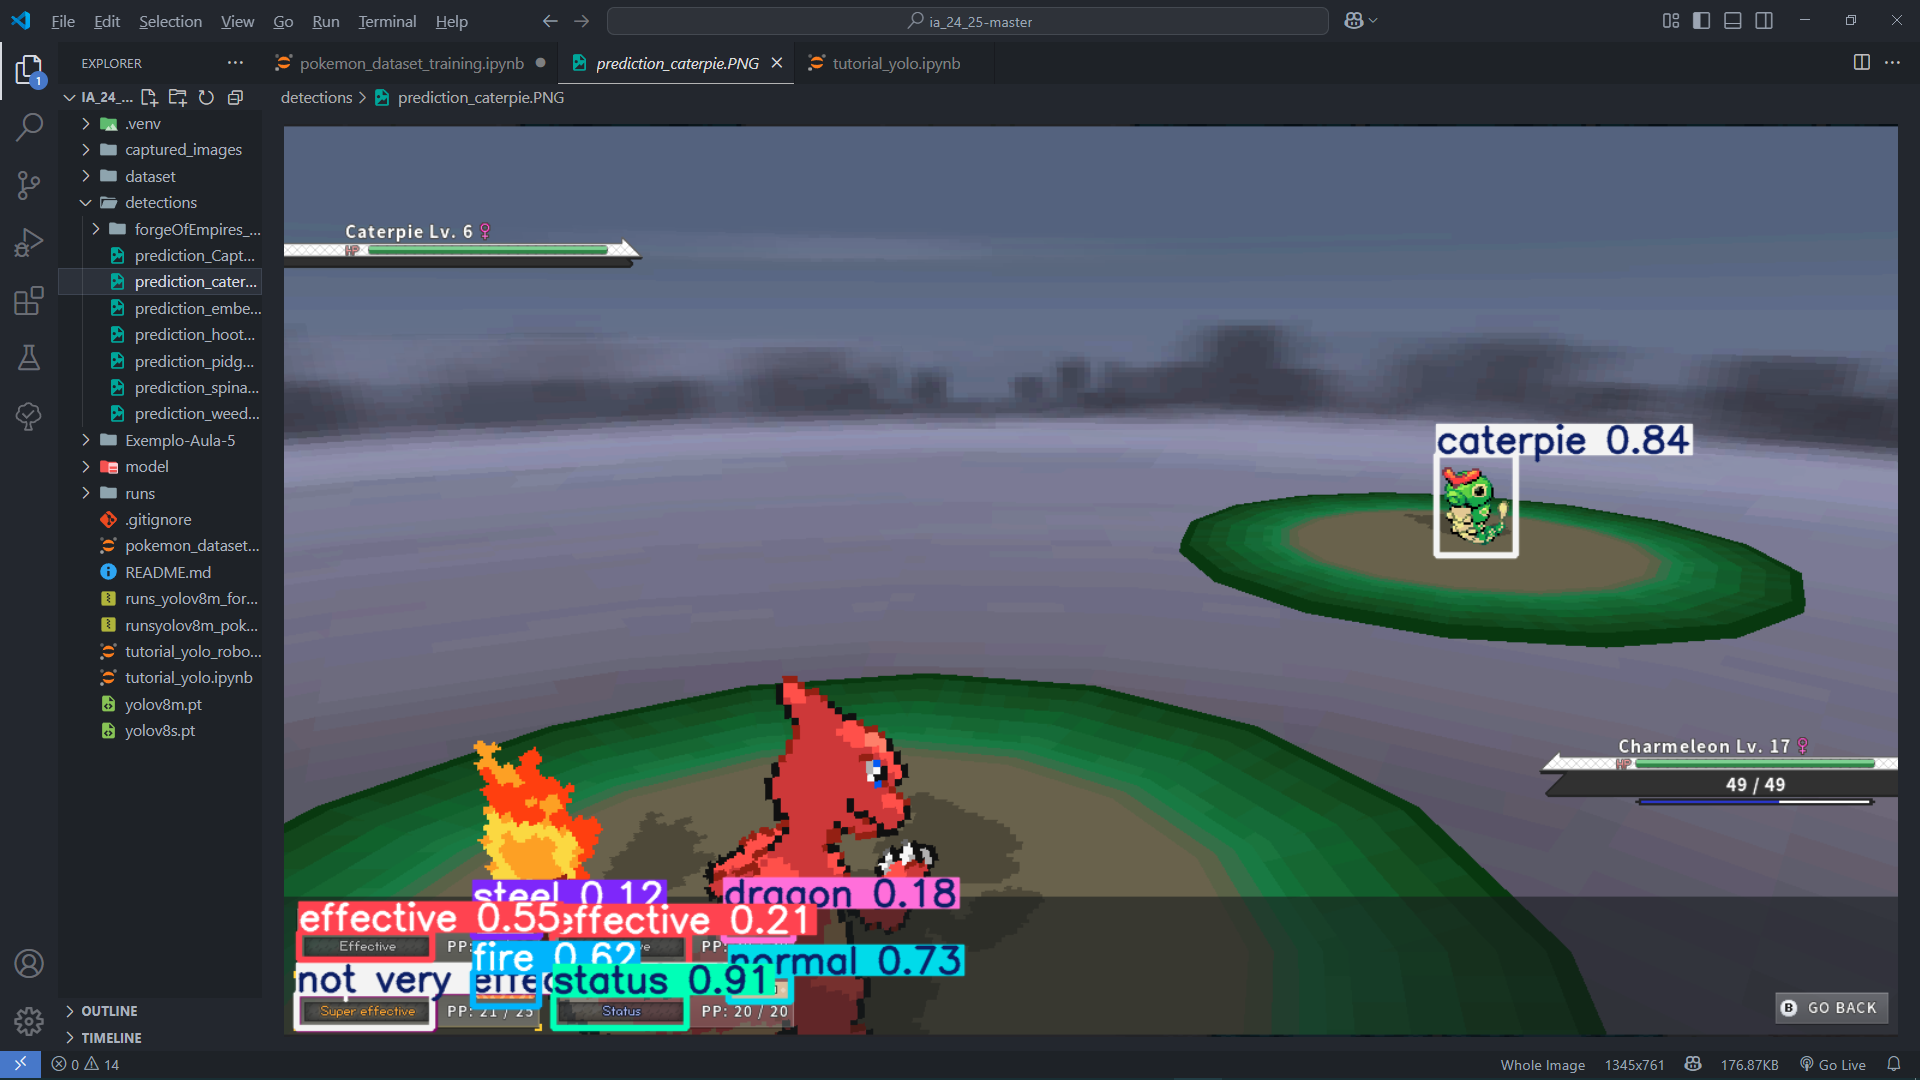
\includegraphics[width=0.7\linewidth]{imagens/primeiro_modelo_exemplo.png}
    \caption{Imagem resultante do primeiro modelo para o PokeMMO}
    \label{fig:primeiro_modelo_exemplo}
\end{figure}

\subsubsection{Segundo Modelo}
Mesmo com os resultados satisfatórios do primeiro modelo treinado, decidiu-se treinar uma nova versão do modelo, mas desta vez com o \textit{YOLOv8x}, que é a melhor versão oferecida pelo \textit{YOLOv8}, no entanto, como o grupo não tinha a capacidade de realizar um treino com esta versão, então recorreu-se à plataforma Kaggle, que permite a execução de notebooks online, possibilitando assim o treinamento de modelos mais pesados.

Num ponto de vista prático, não se conseguiu ver muitas diferenças entre a versão $m$ e a versão $x$ do \textit{YOLOv8}, as imagens devolvidas pelo modelo continuavam a ter um resultado bastante satisfatório, mas não ausente de falsos positivos nem falsos negativos, e também não pareceu haver uma diminuição da ocorrência dos mesmos. No entanto, após tentar levar este modelo para um ambiente de produção, o modelo quase não funcionava, como foram treinadas imagens só com o ecrã de combate, ignorando o resto da interface, o modelo pouco conseguia prever, as informações estavam bastante pequenas para o modelo conseguir detetar, para além de haver muita movimentação tanto da câmara do jogo, como do sprite do Pokémon adversário, dificultando ainda mais a previsão.

Infelizmente não existe forma de aumentar o tamanho do ecrã de batalha nas definições do jogo, e muito provavelmente o problema iria continuar a ocorrer mesmo que se treina-se um novo modelo mas desta vez com imagens do ecrã todo, pois  muitas das informações a recolher já eram pequenas no dataset original, sendo a principal fonte de falsos negativos, logo ao treinar um novo dataset com a totalidade do ecrã pouco iria resolver, portanto decidiu-se trocar de jogo.

\subsection{Modelos para o Pokémon HeartGold}
\subsubsection{Primeiro Modelo}
Após analisar os problemas dos modelos anteriores, chegou-se à conclusão que a série de jogos Pokémon continuava a ser uma boa escolha para o trabalho a desenvolver, o grupo precisava apenas escolher um jogo que se iria adaptar melhor às limitações dos modelos de imagens, então decidiu-se criar um novo dataset mas desta vez para o jogo Pokémon HeartGold, pois como este é um jogo de Nintendo DS, o grupo vai estar sempre limitado à resolução nativa do ecrã do Nintendo DS, e como esta consola tinha um ecrã sensível ao toque, permitia uma fácil execução num ambiente de produção.

Após realizar a recolha, etiquetagem e o treino com o modelo \textit{YOLOv8x}, os resultados obtidos foram bastante satisfatórios. O modelo demonstrou um desempenho muito consistente, com uma taxa reduzida de erros. No entanto, identificou-se um problema recorrente na deteção do botão de "luta". Sempre que o fundo da imagem era predominantemente preto, o modelo tendia a reconhecer essas áreas como sendo o botão de "luta", mesmo quando este não estava presente. Apesar dessas deteções apresentarem geralmente um nível de confiança baixo, e por isso terem impacto reduzido num ambiente de produção, o grupo considerou importante perceber a origem do erro.

Após discutir com o professor da unidade curricular, concluiu-se que o modelo não estava a aprender a identificar o botão com base na cor, mas sim na sua forma retangular. Assim, qualquer área escura com formas semelhantes acabava por ser identificada erroneamente. Para mitigar este tipo de erro, optou-se por aplicar técnicas de \textit{data augmentation}, que permitiram aumentar a robustez do modelo e melhorar a sua capacidade de generalização. As técnicas utilizadas estão descritas com mais detalhe na Secção \ref{data_augmentation}

\begin{figure}[h]
    \centering
    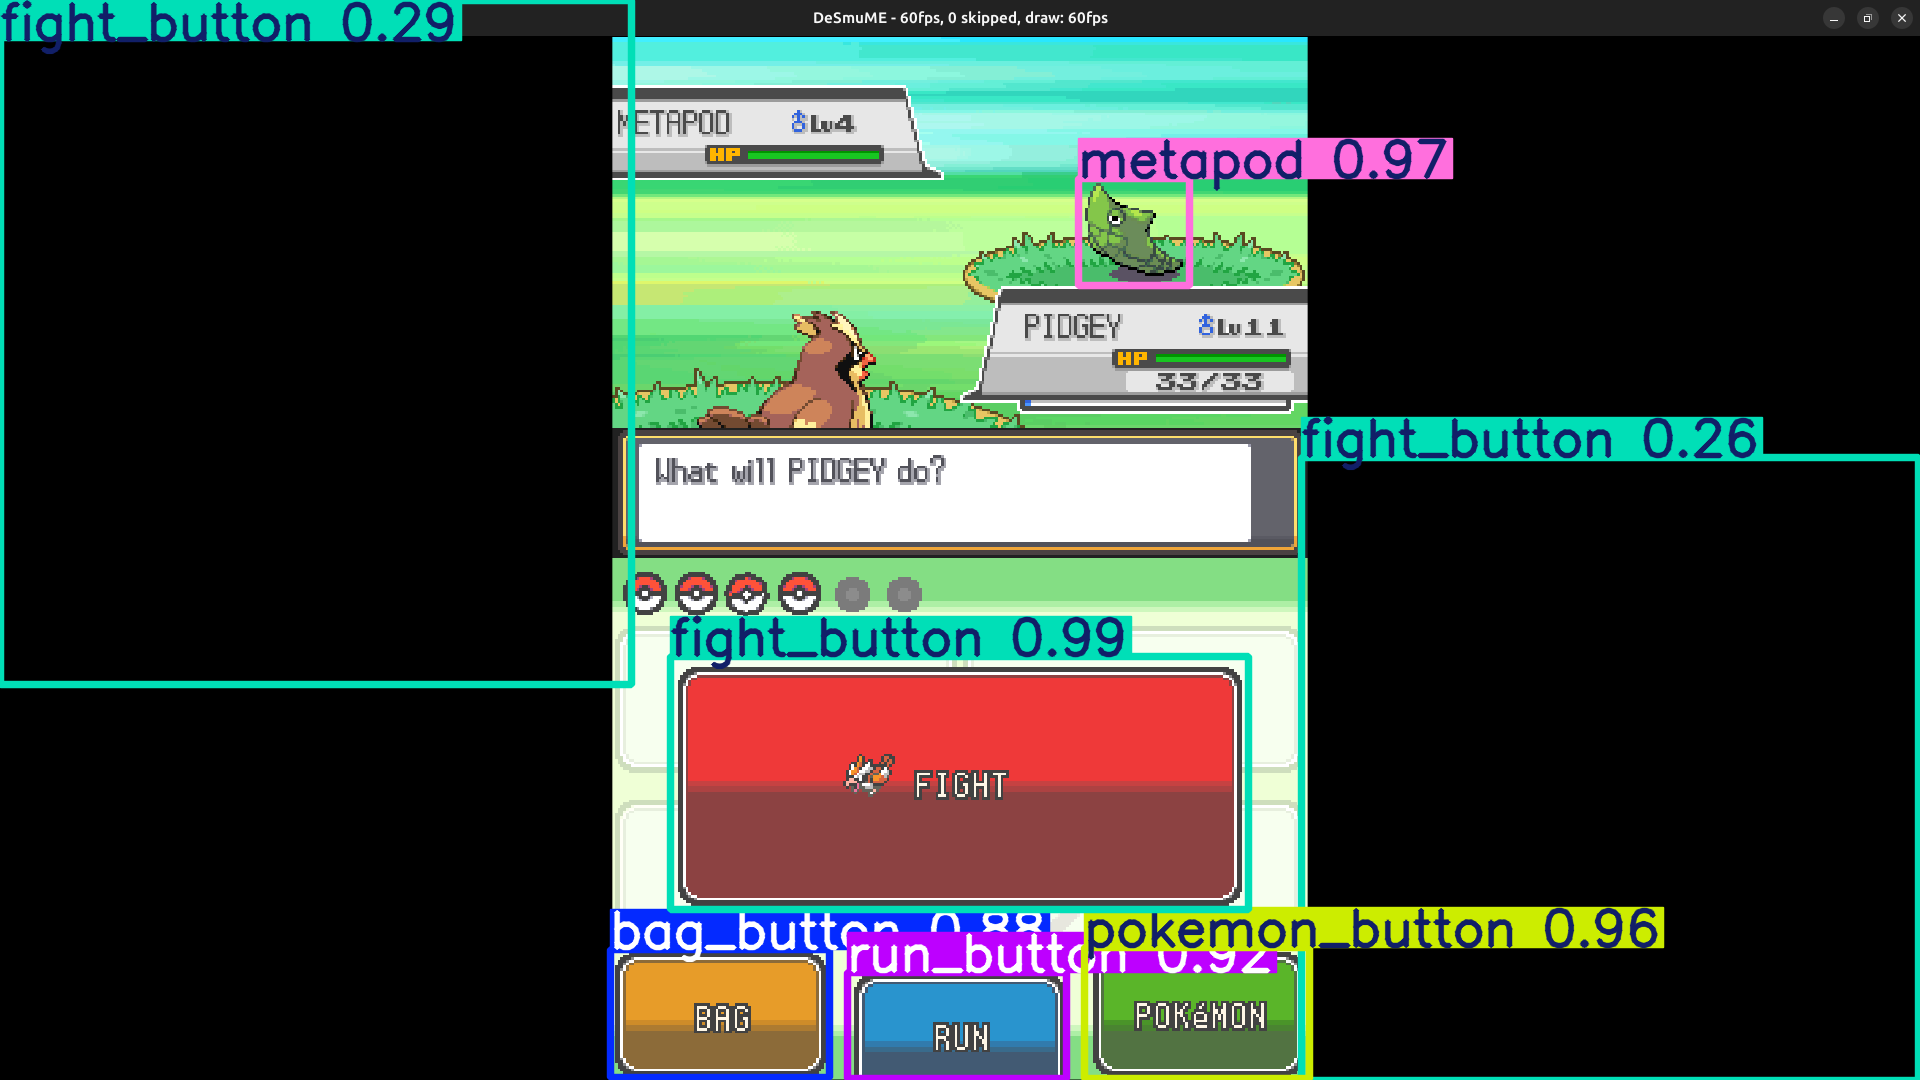
\includegraphics[width=0.8\linewidth]{imagens/phg_fight_button.png}
    \caption{Informações recolhidas do primeiro modelo do Pokémon HeartGold}
    \label{fig:phg_primeiro_modelo}
\end{figure}

Nesta primeira versão do dataset apenas etiquetou-se no roboflow o tipo dos ataques, e não o ataque como um todo, logo o modelo não sabe que ataque está a usar, então para implementar esta primeira versão do modelo, que até então era para ser a definitiva, num ambiente de produção, fez-se um dataset em formato \textit{csv} com a efetividade dos determinados tipos de ataques contra alguns Pokémons presentes no dataset, e treinou-se uma árvore de decisão que iria escolher o ataque que o Pokémon iria usar contra o adversário consoante o tipo do ataque. Como não se sabe o que o ataque faz, esta abordagem acaba por ter vários problemas no combate, porque muitas vezes o modelo previa um determinado ataque como o melhor contra o Pokémon adversário, no entanto, como apenas levou o tipo do ataque em consideração, estava apenas a aplicar buffs (Bónus) a si mesmo ou debuffs (penalizações) ao inimigo, não infringindo dano.

\begin{figure}[h]
    \centering
    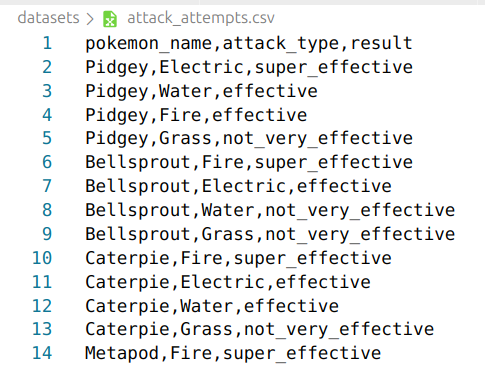
\includegraphics[width=0.5\linewidth]{imagens/dataset_ataques.png}
    \caption{Dataset de efetividade de tipos}
    \label{fig:phg_segundo_modelo}
\end{figure}

\subsubsection{Modelo Final}
Nesta versão do modelo, para além da aplicação de técnicas de \textit{data augmentation}, decidiu-se também recolher mais informações das lutas. Para isso, procedeu-se à identificação dos níveis dos Pokémons em batalha, bem como os nomes dos ataques, com o objetivo de localizar as áreas onde esses elementos estavam presentes. Posteriormente, recorreu-se a uma ferramenta de reconhecimento ótico de caracteres (OCR) para ler essas áreas e, assim, permitir ao bot tomar a melhor decisão com base na informação extraída.

Inicialmente, foi testado o \textbf{Tesseract}, um motor de OCR de código aberto. No entanto, este mostrou-se ineficaz na leitura de texto pixelizado, apresentando resultados fracos na identificação do conteúdo do ecrã.

Seguidamente, utilizou-se o \textbf{EasyOCR}, uma biblioteca de OCR baseada em deep learning, que oferece suporte a múltiplas línguas e é conhecida pela sua simplicidade de utilização. Embora ainda apresentasse alguns erros na leitura dos nomes dos Pokémon e dos ataques, e não conseguisse identificar corretamente os níveis dos Pokémons, representou uma melhoria significativa em relação ao \textit{Tesseract}.

Por fim, foi experimentado o \textbf{Granite}, uma solução mais avançada de OCR baseada em modelos modernos de visão por computador. Contudo, os resultados obtidos não trouxeram melhorias relevantes face ao \textit{EasyOCR} e o tempo de execução era significativamente superior. Dado esse fator, optou-se por manter o \textit{EasyOCR} como ferramenta principal para esta tarefa.

Devido à elevada variabilidade e frequência de erros ortográficos nas informações extraídas, considerou-se inviável treinar um modelo tradicional para a tomada de decisões. Assim, optou-se pela utilização de um modelo de linguagem (LLM) local, executado através do \textit{Ollama}, que permite interpretar e decidir com base em texto imperfeito. Inicialmente foi testado o modelo \textbf{TinyLlama}, mas este não seguia de forma fiável as instruções fornecidas. Portanto decidiu-se experimentar os modelos \textbf{Phi2}, \textbf{Phi4}, \textbf{Deepseek-v2}, sendo que, no final, o modelo que melhor se adequou às exigências do projeto, seja ao nível de respostas como ao nível de desempenho, foi o \textbf{Mistral}.

Embora o modelo ainda apresente algumas limitações na interpretação de certas entradas, os resultados obtidos são, de forma geral, bastante satisfatórios. A sua capacidade de lidar com dados ruidosos e tomar decisões coerentes torna-o suficientemente robusto para ser utilizado em ambiente de produção.

\begin{figure}[h]
    \centering
    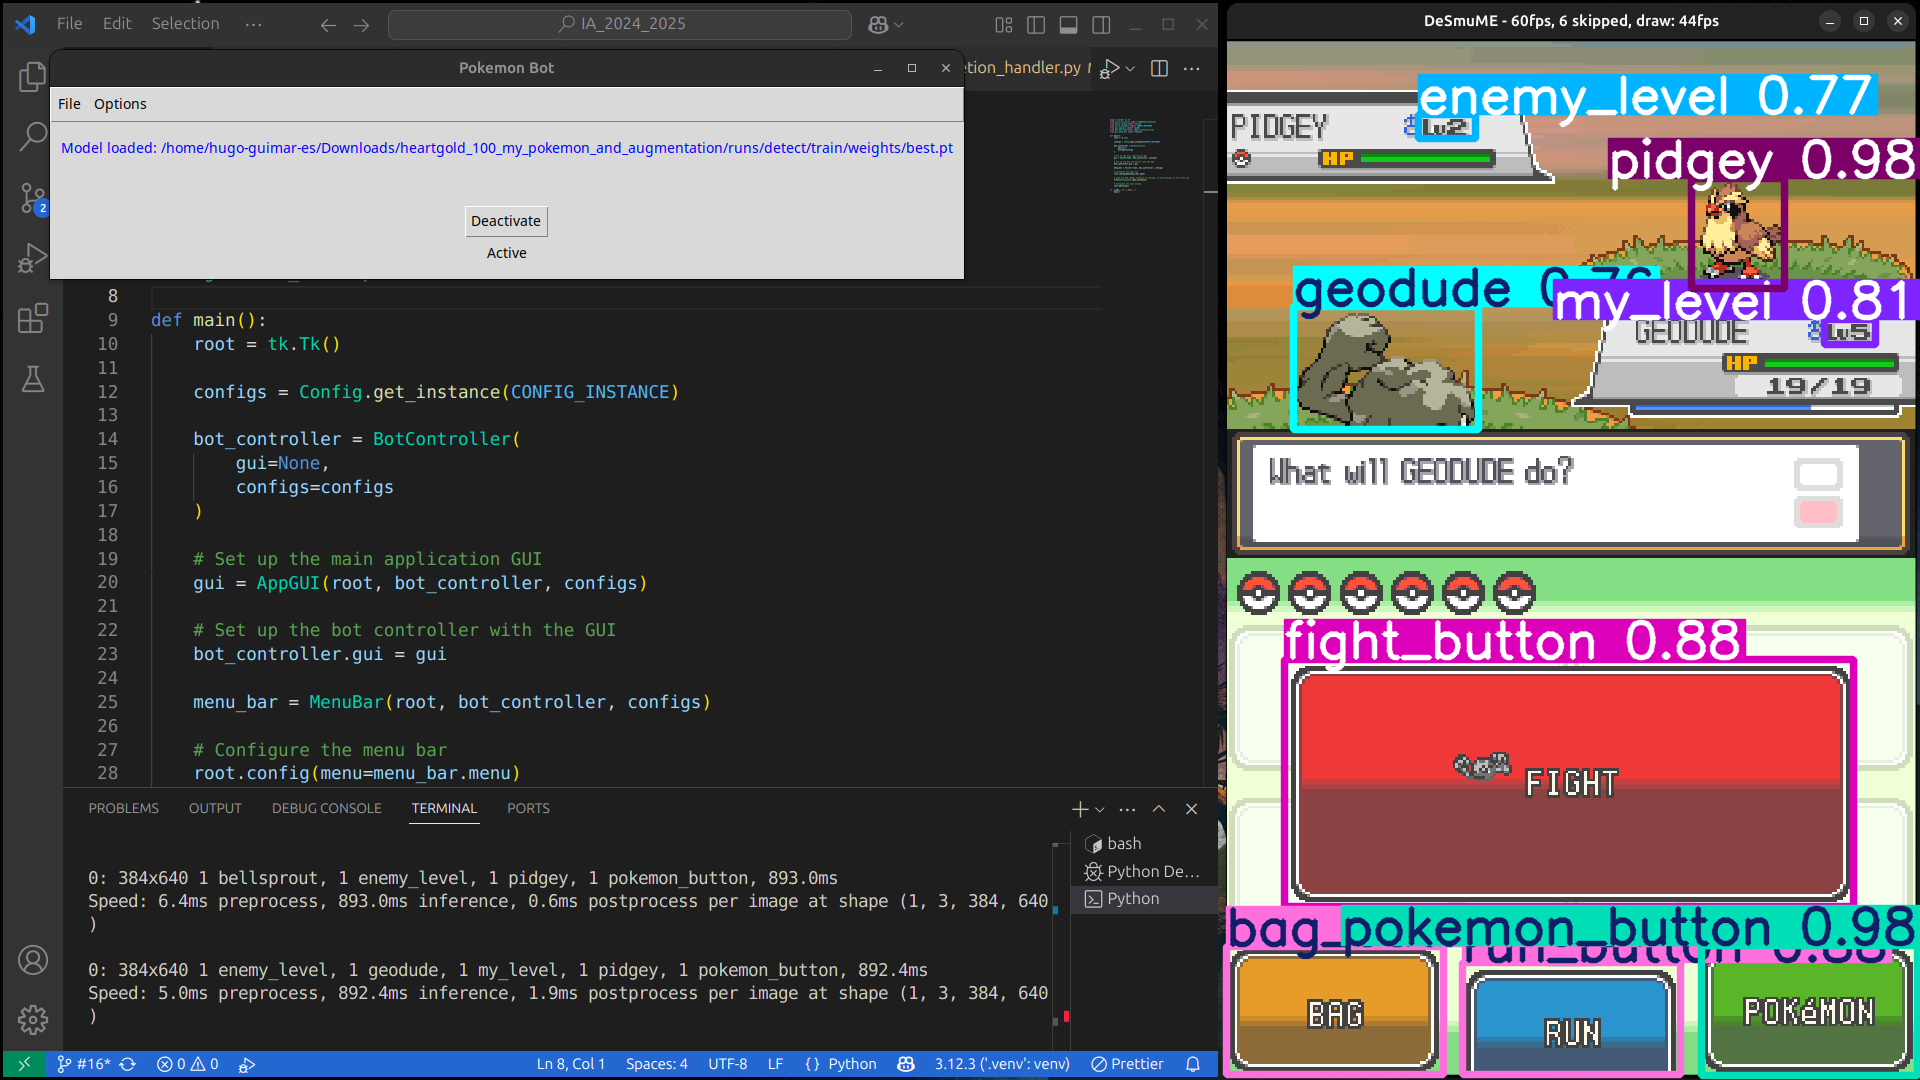
\includegraphics[width=1.0\linewidth]{imagens/informacoes_modelo_final.png}
    \caption{Informações recolhidas pelo modelo final em produção}
    \label{fig:infomacoes_modelo_final}
\end{figure}

% Data Augmentation
\section{Técnicas Utilizadas de Data Augmentation} \label{data_augmentation}

Em muitos projetos de Inteligência Artificial, a qualidade e a quantidade dos dados disponíveis têm um impacto direto no desempenho do sistema. Contudo, nem sempre é viável recolher grandes volumes de dados diversificados. Para contornar essa limitação, é comum recorrer a técnicas de \textit{Data Augmentation} (aumento de dados), que consiste em gerar novas amostras a partir das existentes, através da aplicação de transformações específicas.

Esta abordagem permite enriquecer o conjunto de dados original, aumentando a sua variedade e tornando o modelo mais robusto a variações. Assim, o \textit{data augmentation} contribui para melhorar a capacidade do sistema de reconhecer padrões e lidar com situações diferentes das observadas inicialmente.

Para o projeto desenvolvido foram utilizadas as seguintes abordagens de \textit{Data Augmentation}

\subsection{Inserção de Imagens em Fundos Diferentes}

Depois que se mudou de jogo para o \textit{Pokémon HeartGold}, começaram a surgir alguns problemas, onde o modelo detetava botões em locais onde os mesmos não existiam, nem sequer era percetível a presença de um botão nesse lugar. Um exemplo disso são as bordas escuras à esquerda e à direita do jogo, onde o modelo reconhecia botões de combate, apesar de não haver cor nem texto indicativo da presença de um botão. Para um ser humano, é óbvio que ali não poderia estar um botão de combate, mas o modelo estava a identificar padrões que levavam a essa deteção incorreta.

Após algum falar com o professor da disciplina e várias tentativas, percebeu-se que o modelo não estava a aprender a identificar os botões de combate com base na sua cor ou texto, como era o esperado, mas sim apenas pelo seu formato retangular. Por esse motivo, o modelo detetava falsos positivos em regiões onde observava formas semelhantes, como os fundos escuros das bordas.

Para resolver este problema, decidiu-se recorrer a técnicas de \textit{augmentation}, onde os elementos que se pretendem identificar foram recortados e inseridos em fundos de cores diferentes, com o objetivo de forçar o modelo a aprender que os botões devem ser identificados pela sua cor e características visuais, e não apenas pela forma.

Infelizmente, a plataforma \textit{RoboFlow} não disponibilizava este tipo específico de \textit{Data Augmentation} no momento da realização do projeto, pelo que foi necessário realizar este processo manualmente. Os botões foram recortados com o programa de manipulação de imagens \textit{Gimp} e colados sobre diferentes fundos.


\begin{figure}[h]
    \centering
    
\includegraphics[width=0.5\textwidth]{imagens/augmentation_dark_gray.png}
    \caption{Exemplo de imagem gerada manualmente para \textit{Data Augmentation} no GIMP.}
    \label{fig:data_aug_gimp}
\end{figure}

% Avaliação do Modelo
\section{Avaliação dos Modelos} \label{avaliacoes_dos_modelos}
Para avaliar o desempenho dos modelos de deteção de objetos, foi utilizada a matriz de confusão, e várias métricas padrão na área de Visão Computacional. As principais métricas consideradas foram:

\begin{itemize}
    \item \textbf{Precision (Precisão)}: Mede a proporção de predições corretas entre todas as predições positivas. Um valor elevado indica que o modelo comete poucos falsos positivos.
    
    \item \textbf{Recall (Revocação)}: Mede a proporção de objetos verdadeiros que foram corretamente detetados. Um valor elevado indica que o modelo falha poucas vezes as deteções.
    
    \item \textbf{mAP@50 (Mean Average Precision a 50\% IoU)}: É a média da precisão ao longo de todas as classes, e a mais comum em benchmarks. Deve estar o mais próximo possível de 1.
    
    \item \textbf{mAP@50-95}: É a média da mAP considerando múltiplos limiares de IoU entre 50\% e 95\%, com incrementos de 5\%. Esta métrica é mais exigente e fornece uma avaliação mais abrangente.
    
    \item \textbf{Perdas (Losses)}: Foram monitorizadas as perdas de \textit{box\_loss}, \textit{cls\_loss} e \textit{dfl\_loss} durante o treino e validação. Estas perdas indicam o erro cometido na regressão da caixa delimitadora, na classificação e na distribuição espacial das previsões, respetivamente.
\end{itemize}

%
% Modelos PokeMMO
%
\subsection{Modelos do PokeMMO}
Foram treinados dois modelos com os mesmos parâmetros. Ambos foram treinados durante 100 épocas. No entanto, um dos modelos foi treinado com o \textit{YOLOv8m} e o outro com o \textit{YOLOv8x}, sendo que este último é, teoricamente, uma versão superior à versão \textit{m}. Como tal, requer mais tempo de treino e maior capacidade computacional. Assim, será realizada uma avaliação onde se irá comparar os dois modelos iniciais, de forma a determinar se o tempo e os recursos investidos no treino da versão \textit{x} são justificáveis e se faz sentido optar por esta versão nos treinos de modelos futuros.

\begin{figure}[h]
    \centering
    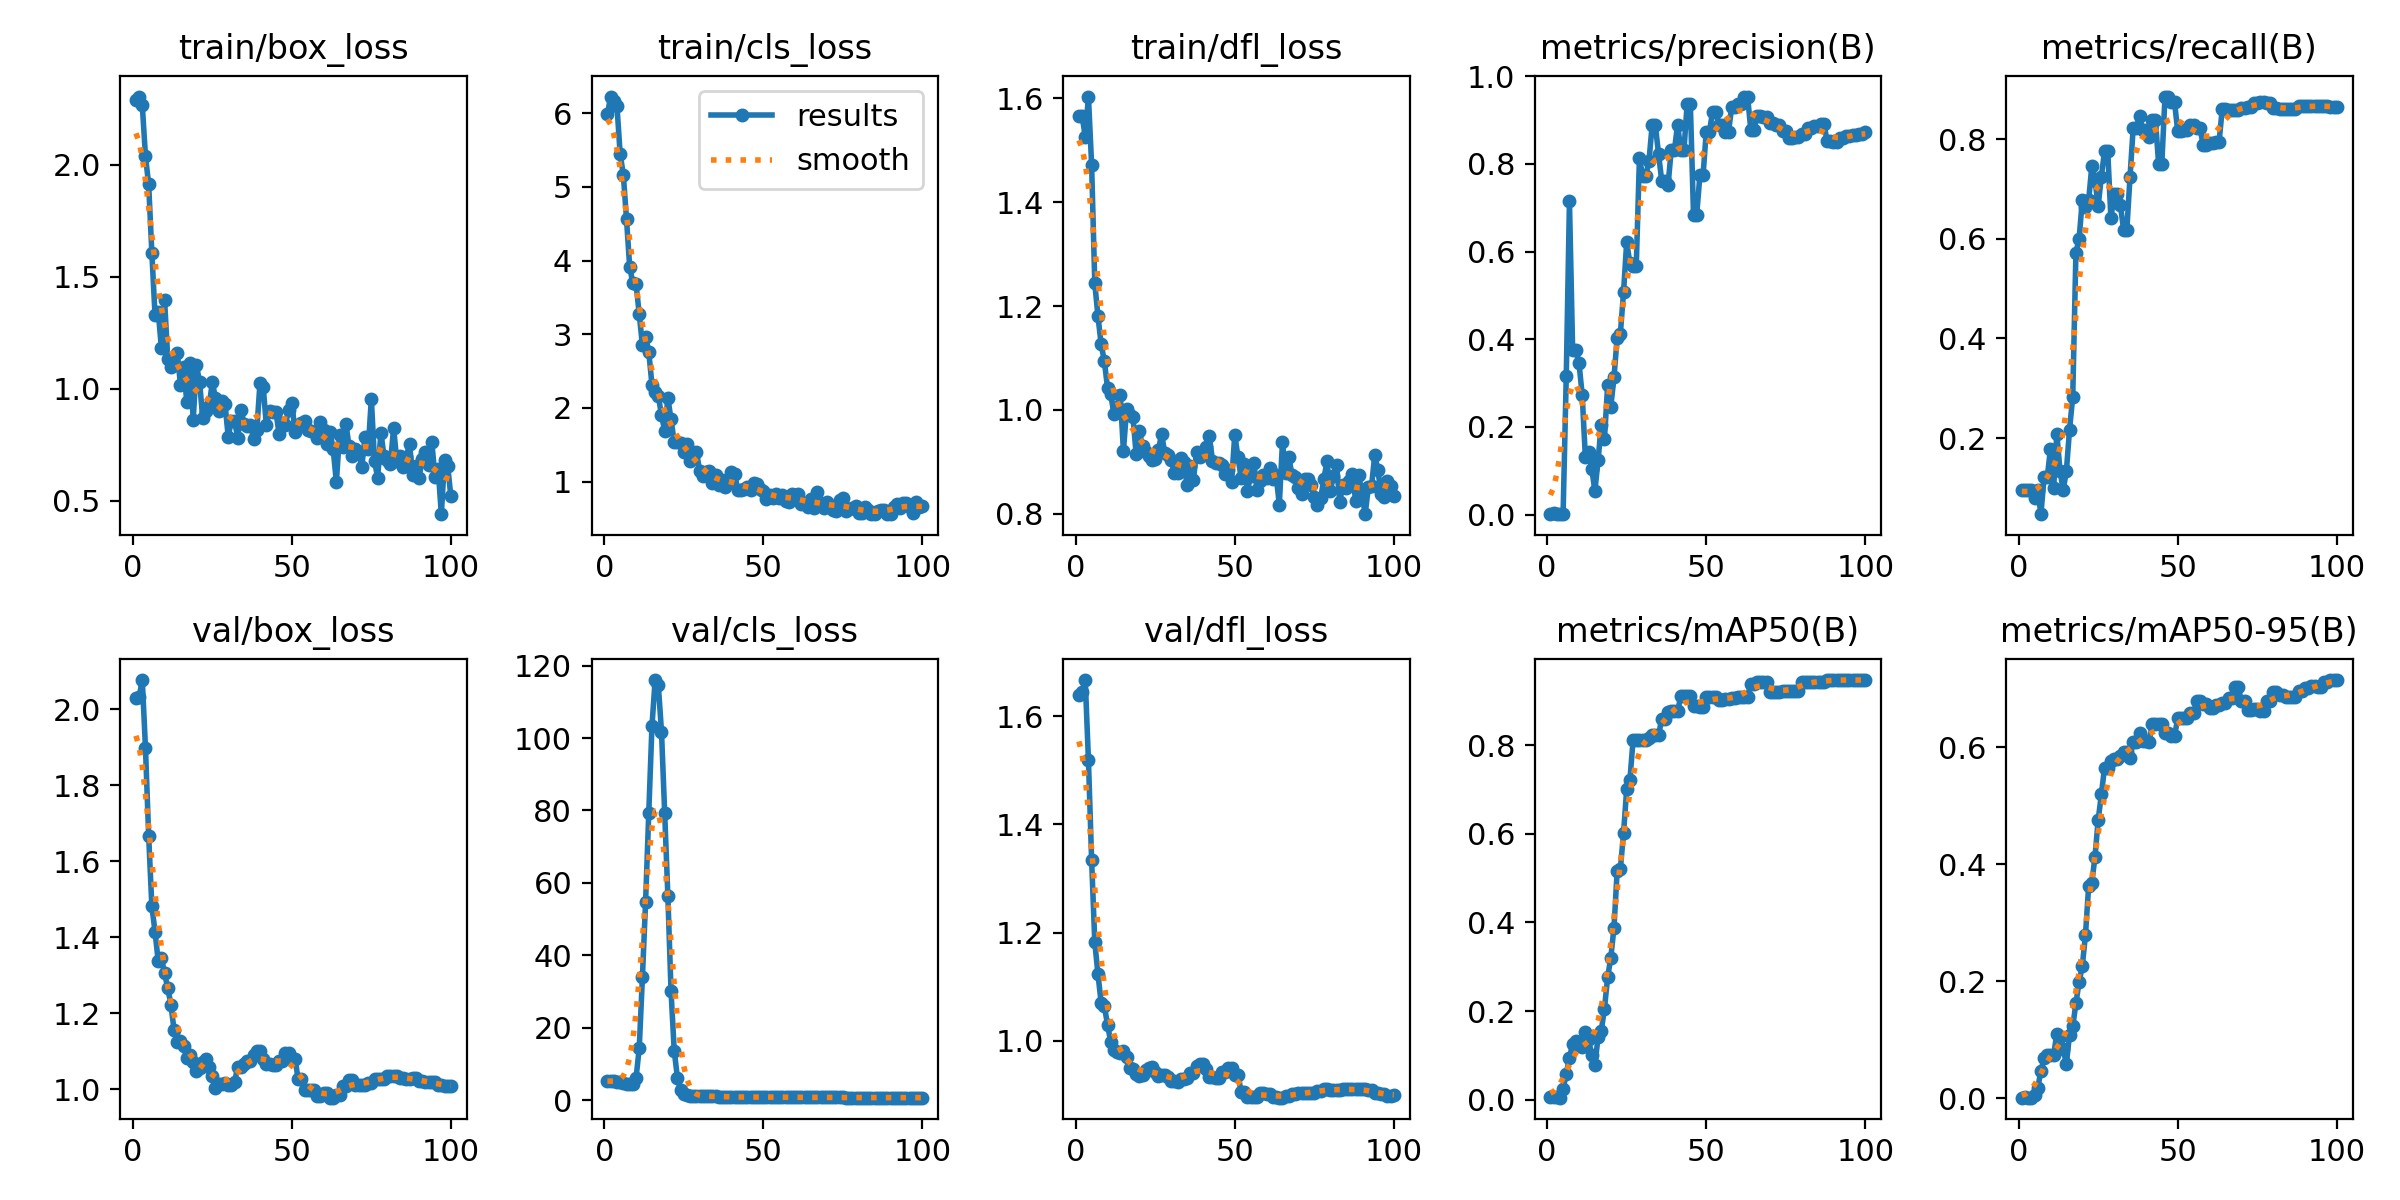
\includegraphics[width=0.7\textwidth]{imagens/results_modelom.png}
    \caption{Gráficos de desempenho do primeiro modelo criado para o PokeMMO (YOLOv8m).}
    \label{fig:results_modelom}
\end{figure}

\begin{figure}[h]
    \centering
    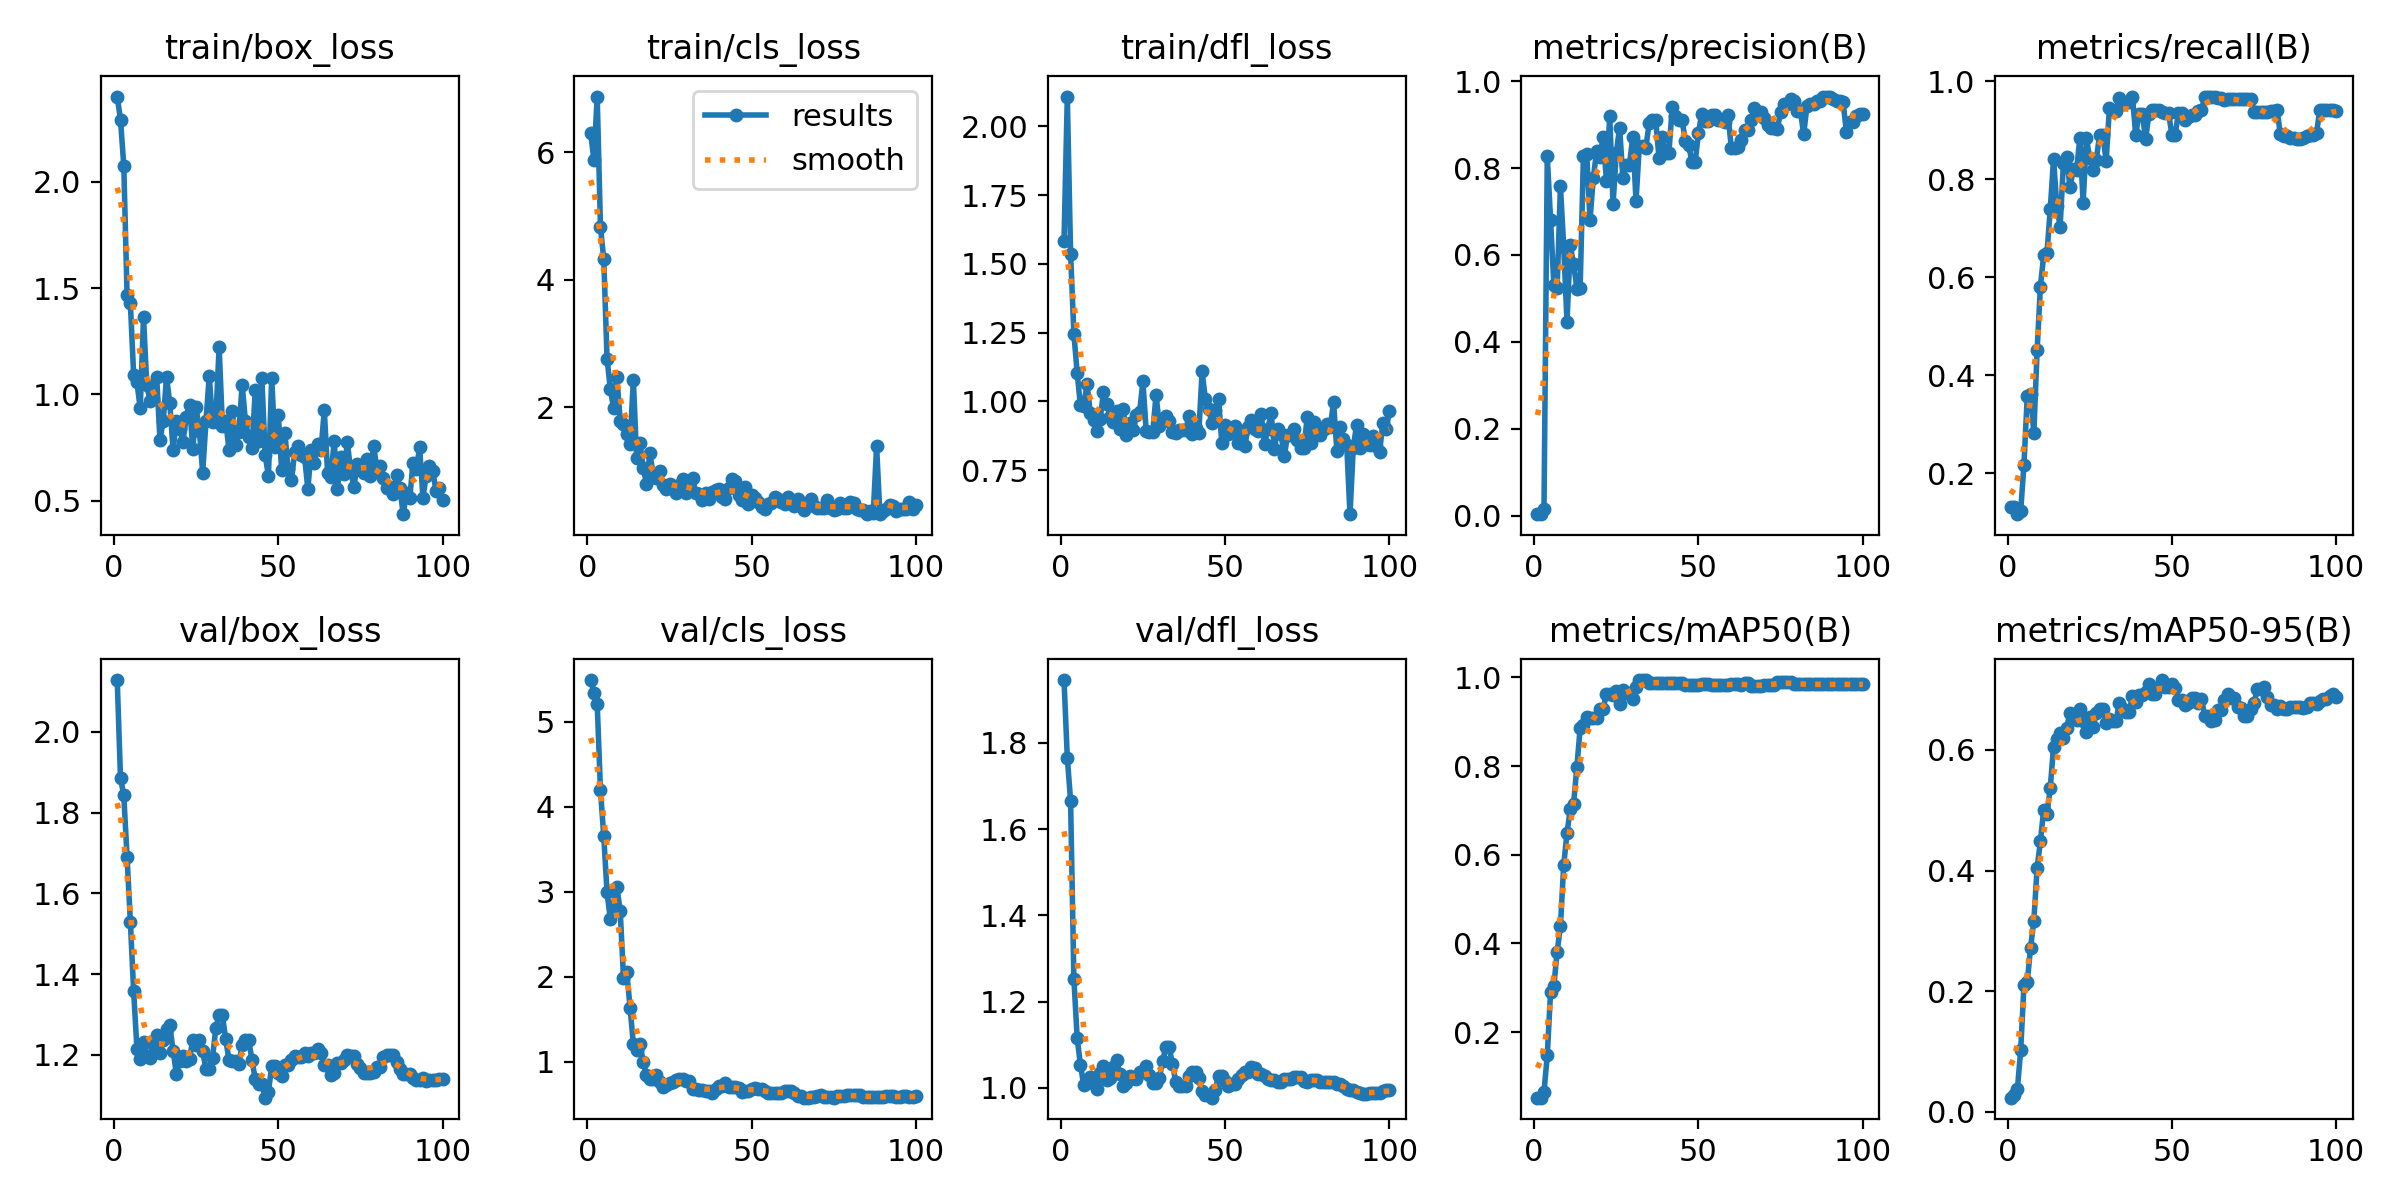
\includegraphics[width=0.7\textwidth]{imagens/results_modelox.png}
    \caption{Gráficos de desempenho do segundo modelo criado para o PokeMMO(YOLOv8x).}
    \label{fig:results_modelox}
\end{figure}

A parir dos gráficos de desempenho de cada modelo nas figuras \ref{fig:results_modelom} e \ref{fig:results_modelox} observa-se que:

\begin{itemize}
    \item As métricas de \textbf{precision} e \textbf{recall} estabilizaram acima dos 90\% em ambos os modelos, mas é possível visualizar que no modelo \textit{x} a linha não oscilou tanto, para além de se ter estabilizando mais cedo acima dos 90\%.
    
    \item O \textbf{mAP@50} aproxima-se de 1.0, o que indica uma excelente performance nas deteções, mais uma vez é possível detetar algumas oscilações no modelo \textit{m}, e uma aproximação de 1.0 mais cedo no modelo \textit{x}.
    
    \item O \textbf{mAP@50-95} estabilizou por volta de 0.7, o que demonstra boa generalização mesmo em critérios mais exigentes.
    
    \item As \textbf{perdas de validação} diminuíram progressivamente e estabilizaram, sem sinais evidentes de overfitting.
\end{itemize}

A partir das métricas analisadas, é possível concluir que o modelo \textit{YOLOv8x} apresentou um desempenho ligeiramente superior ao modelo \textit{YOLOv8m}. Isso é reforçado não apenas pelas curvas mais estáveis e pela convergência mais rápida nas métricas principais, mas também pelas matrizes de confusão, onde se observa que o modelo \textit{m} cometeu mais erros de classificação do que o modelo \textit{x}.

\begin{figure}[h]
    \centering
    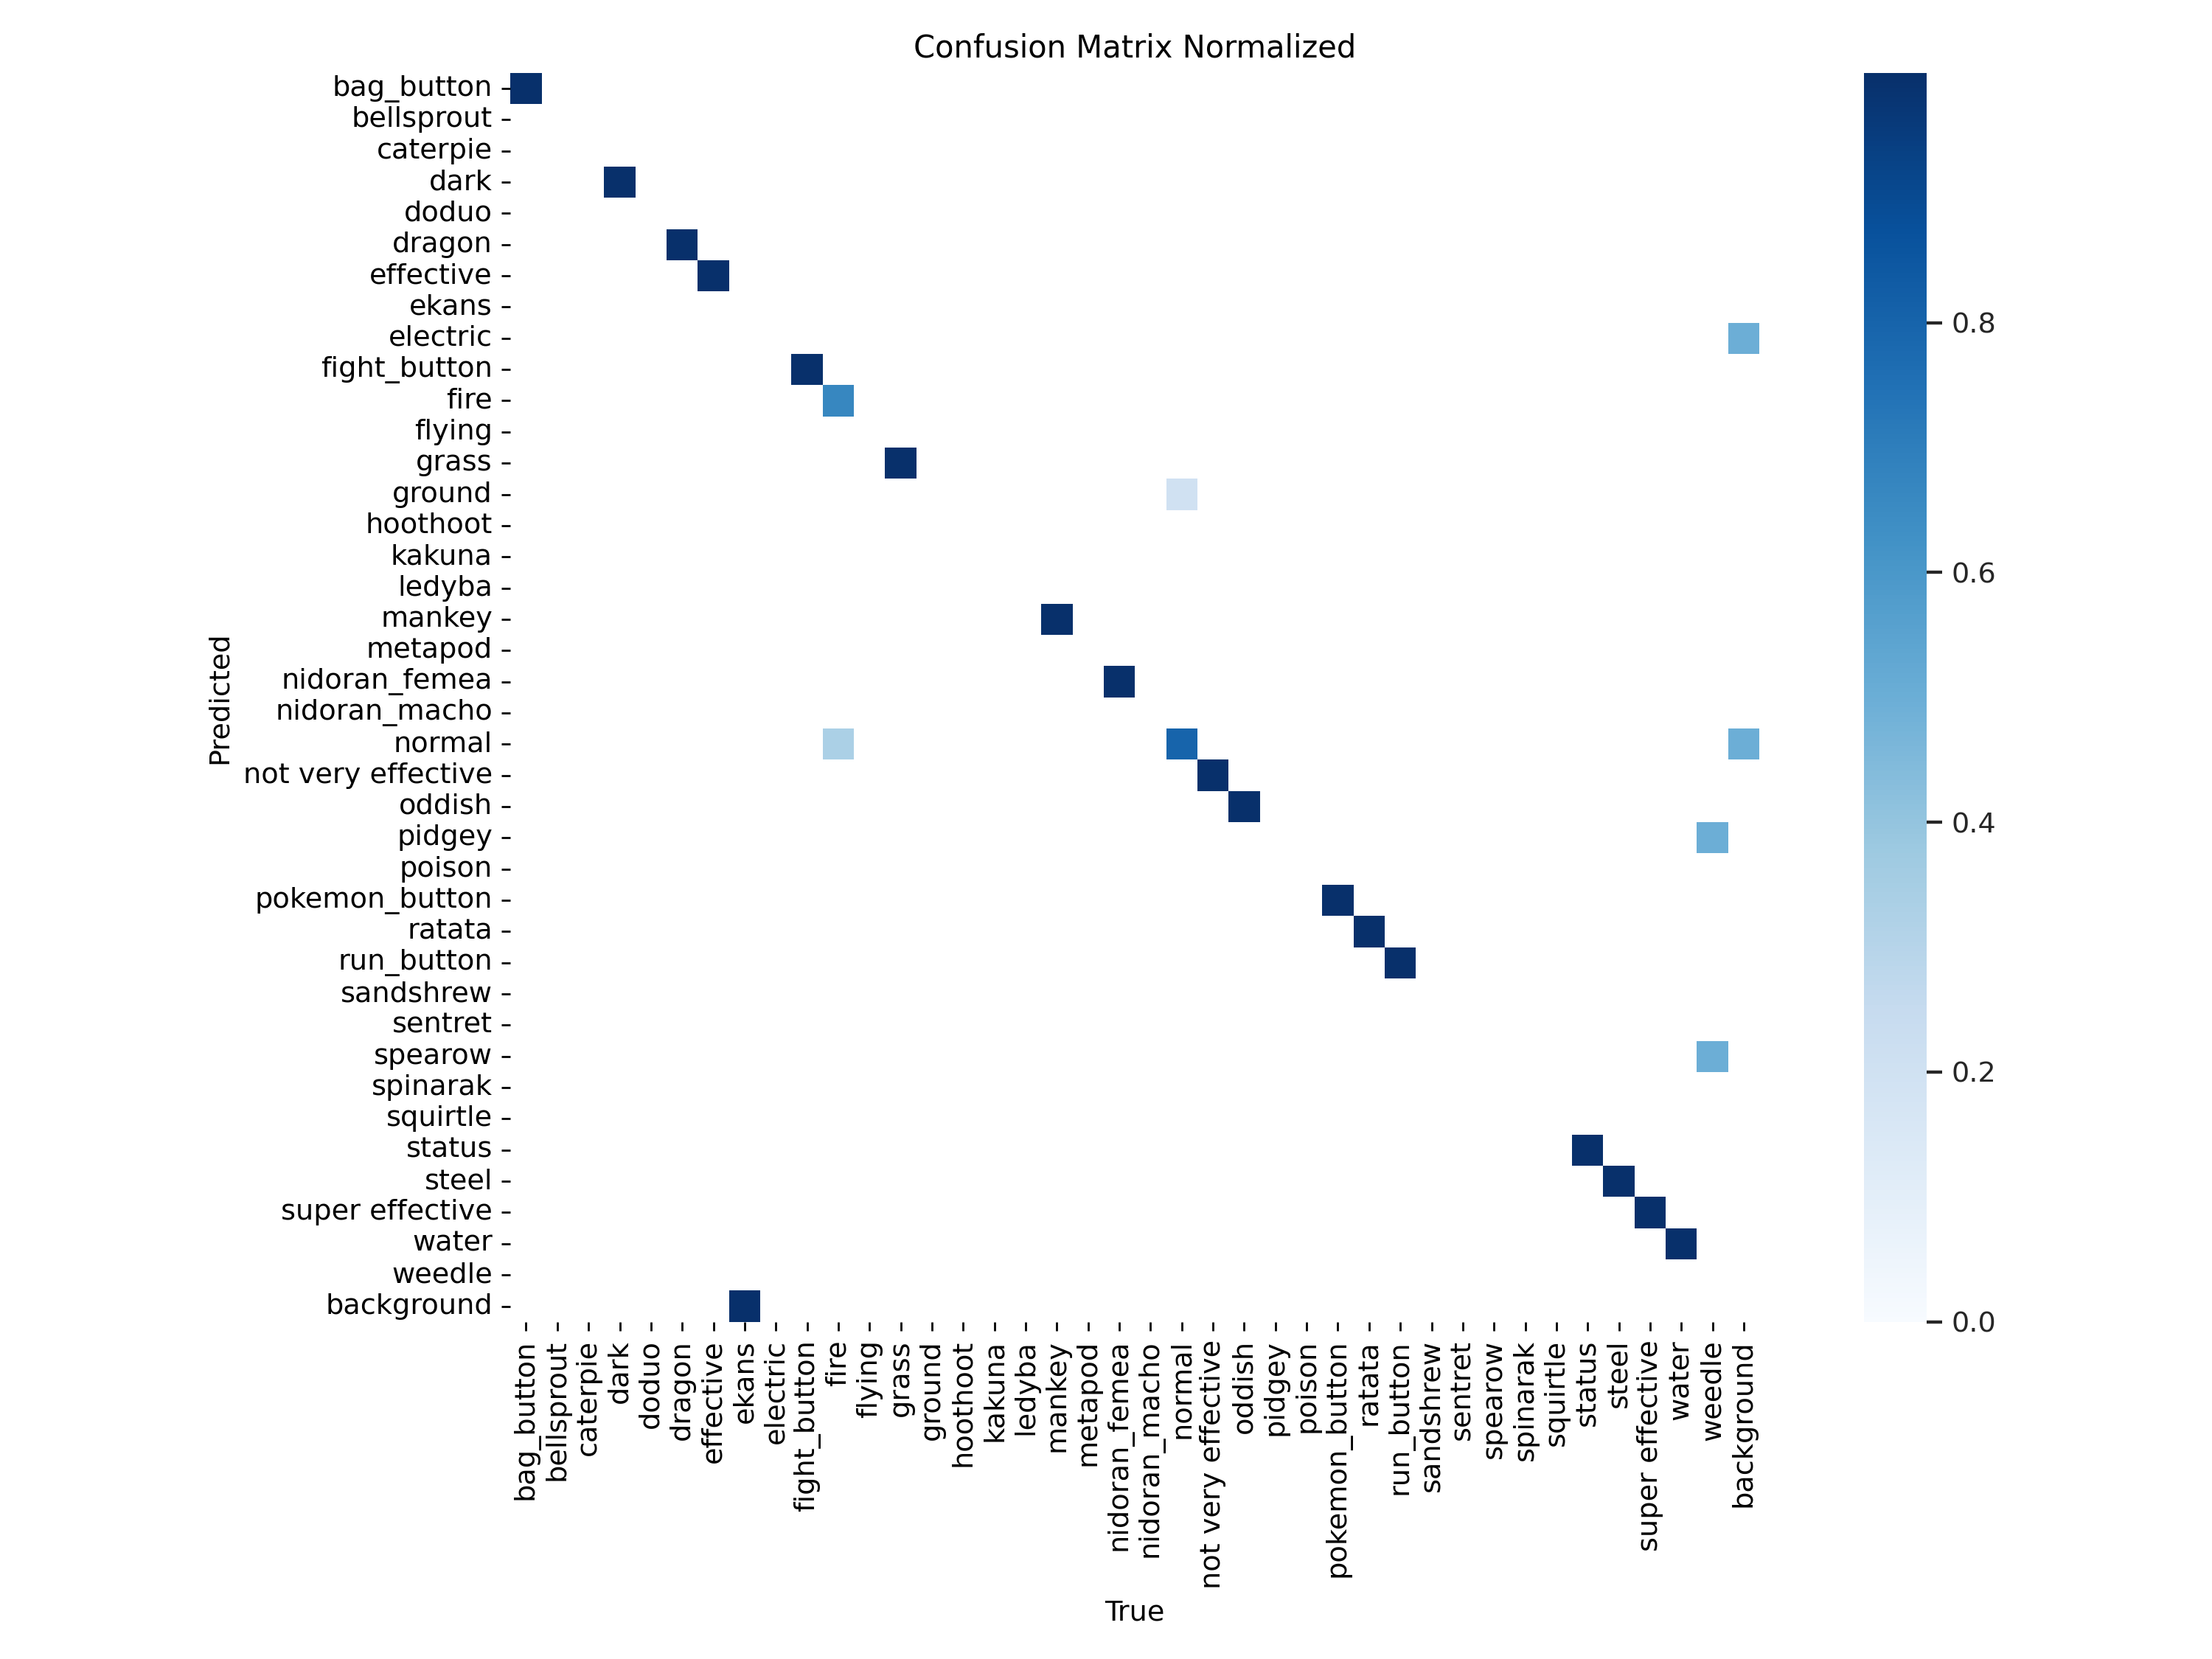
\includegraphics[width=0.65\textwidth]{imagens/confusion_matrix_normalized_modelom.png}
    \caption{Matriz de confusão do primeiro modelo criado para o PokeMMO (YOLOv8m).}
    \label{fig:confusion_matrix_modelom}
\end{figure}

\begin{figure}[h]
    \centering
    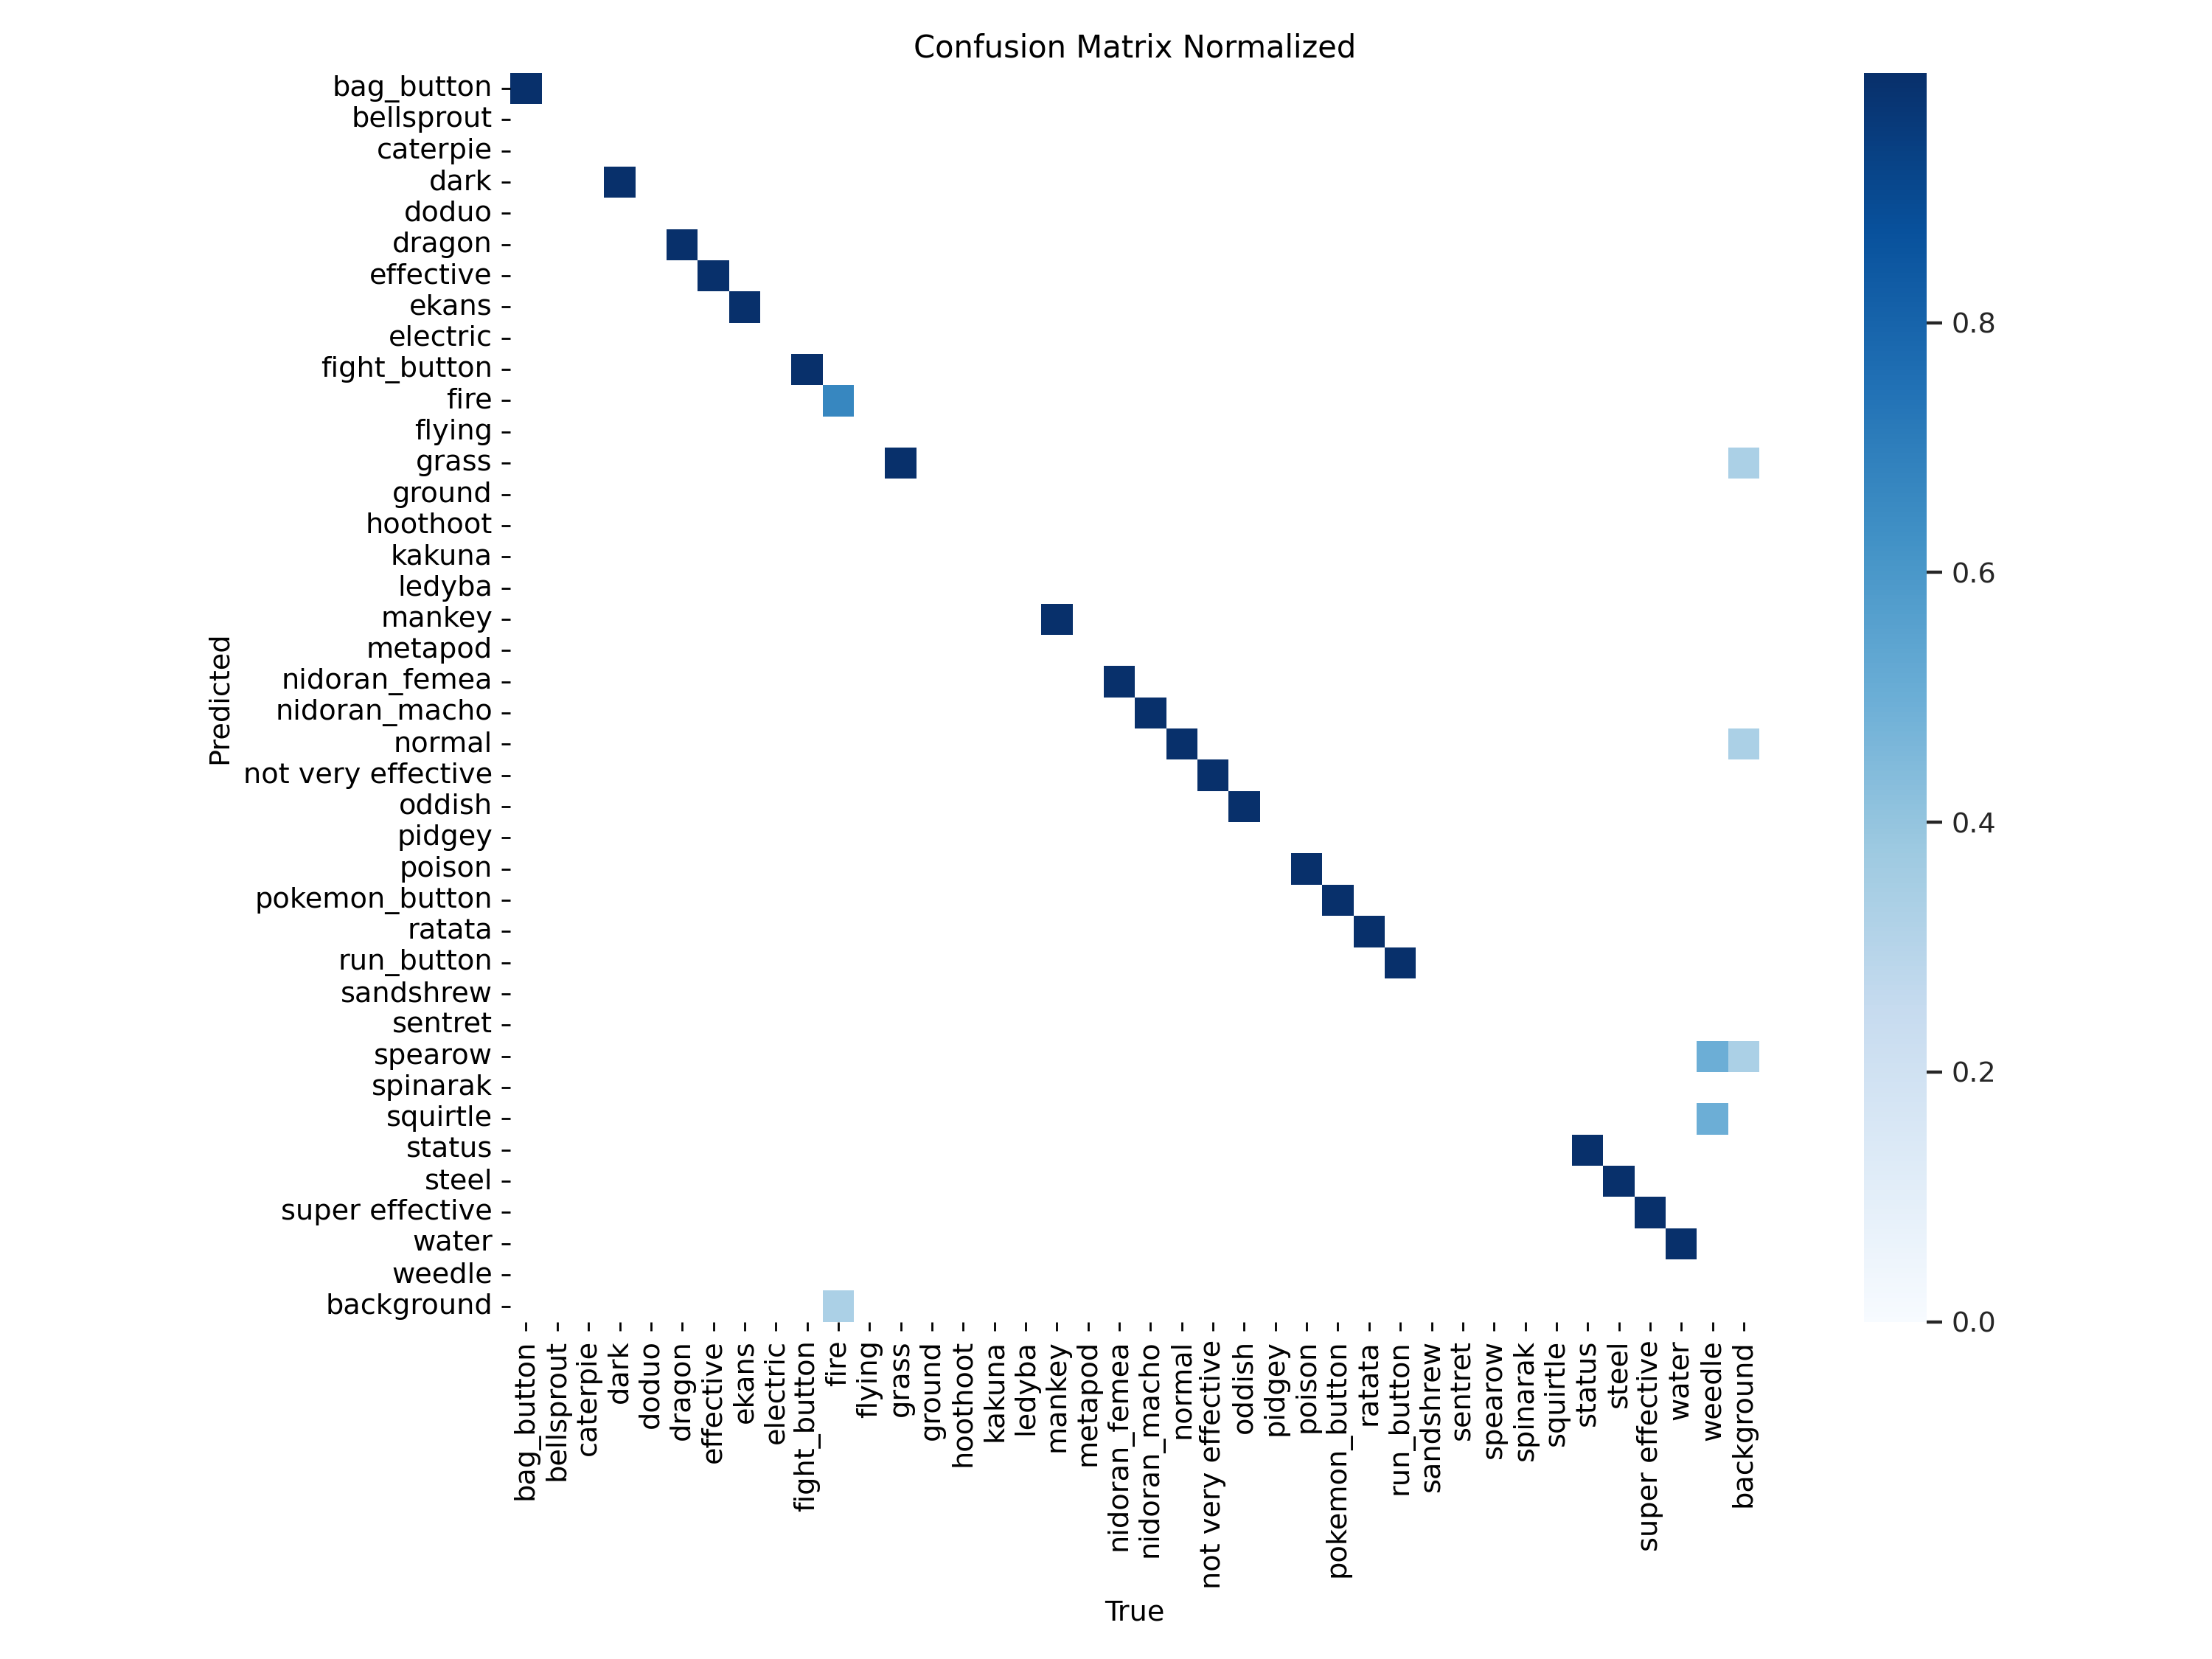
\includegraphics[width=0.65\textwidth]{imagens/confusion_matrix_normalized_modelox.png}
    \caption{Matriz de confusão do segundo modelo criado para o PokeMMO (YOLOv8x).}
    \label{fig:confusion_matrix_modelox}
\end{figure}

Apesar das melhorias não serem extremamente significativas, o modelo \textit{YOLOv8x} demonstrou maior robustez, especialmente na redução de falsos positivos. Por essa razão, decidiu-se utilizá-lo como base para os modelos treinados nas etapas seguintes.



%
% Modelos PokemonHeartGold
%
\subsection{Modelos do Pokémon HeartGold}
Para o jogo Pokémon HeartGold foram treinados vários modelos diferentes, onde a cada modelo era um incremento do modelo anterior, onde eram adicionadas novas classes para identificar objetos diferentes no ecrã. O primeiro modelo foi treinado com um número reduzido de classes, enquanto que o último modelo foi treinado com um conjunto mais completo de classes. Ambos os modelos utilizaram o mesmo modelo (\textit{YOLOv8x}) e foram treinados com 100 épocas, sendo a principal diferença entre os modelos a complexidade e diversidade dos dados de treino, com o último modelo a incluir técnicas de \textit{data augmentation} para melhorar a generalização.

Deste modo, será realizada uma análise comparativa entre os dois modelos, mesmo reconhecendo que os conjuntos de dados e os objetivos de cada um não são exatamente equivalentes. O objetivo desta comparação é perceber se, com o aumento da complexidade, se houve uma evolução significativa na capacidade de deteção e desempenho geral do sistema.

\begin{figure}[h]
    \centering
    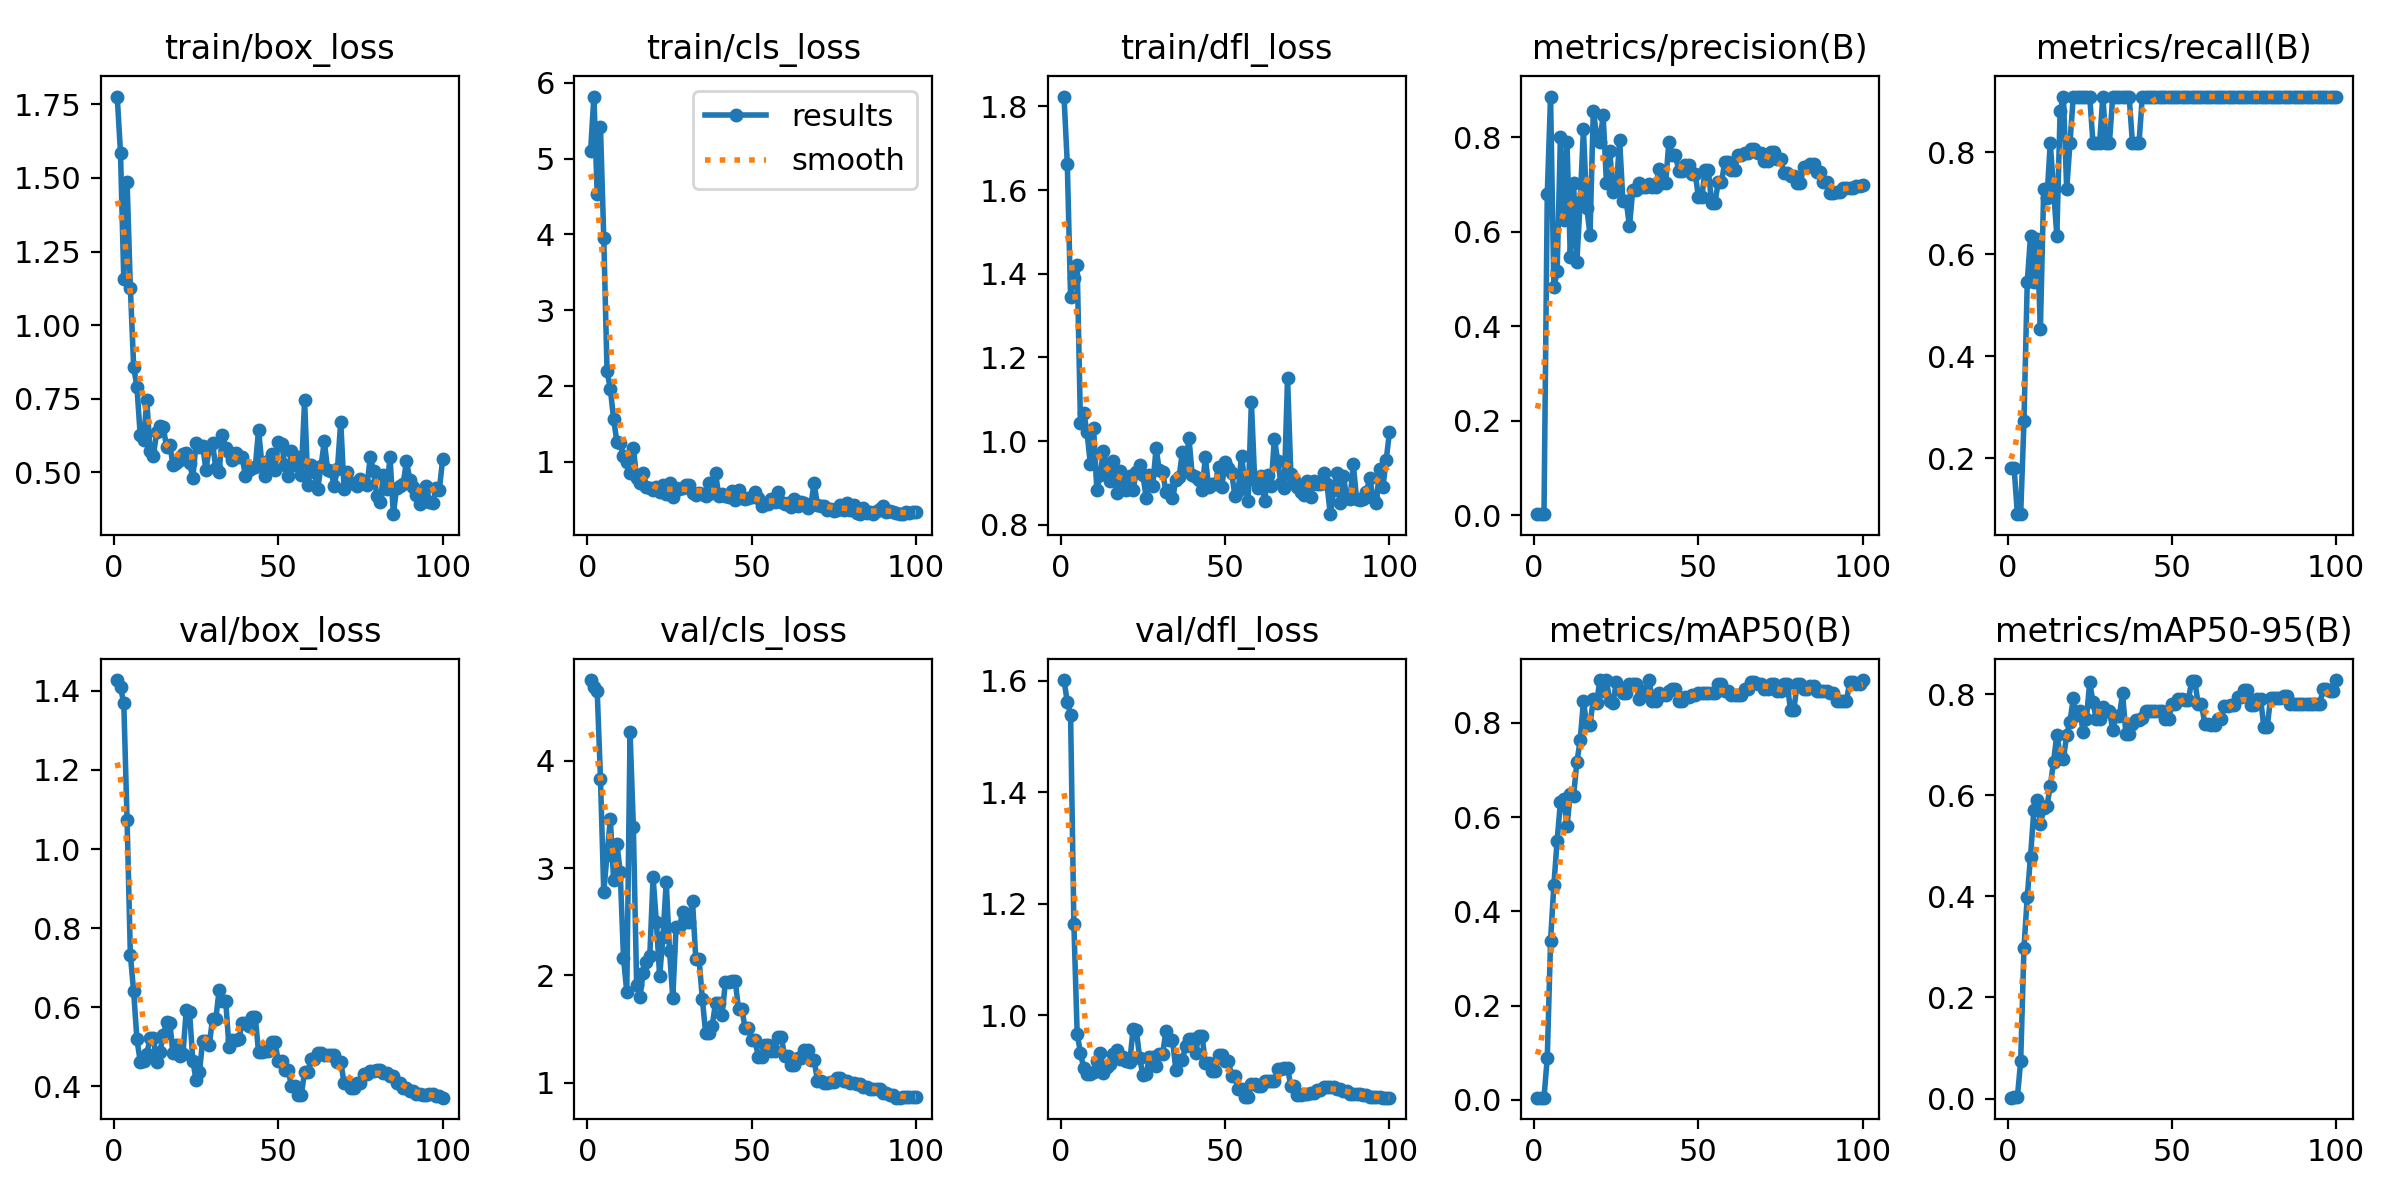
\includegraphics[width=0.80\textwidth]{imagens/results_primeiro_modelo.png}
    \caption{Gráficos de desempenho do primeiro modelo criado para o Pokémon HeartGold.}
    \label{fig:results_primeiro_modelo}
\end{figure}

\begin{figure}[h]
    \centering
    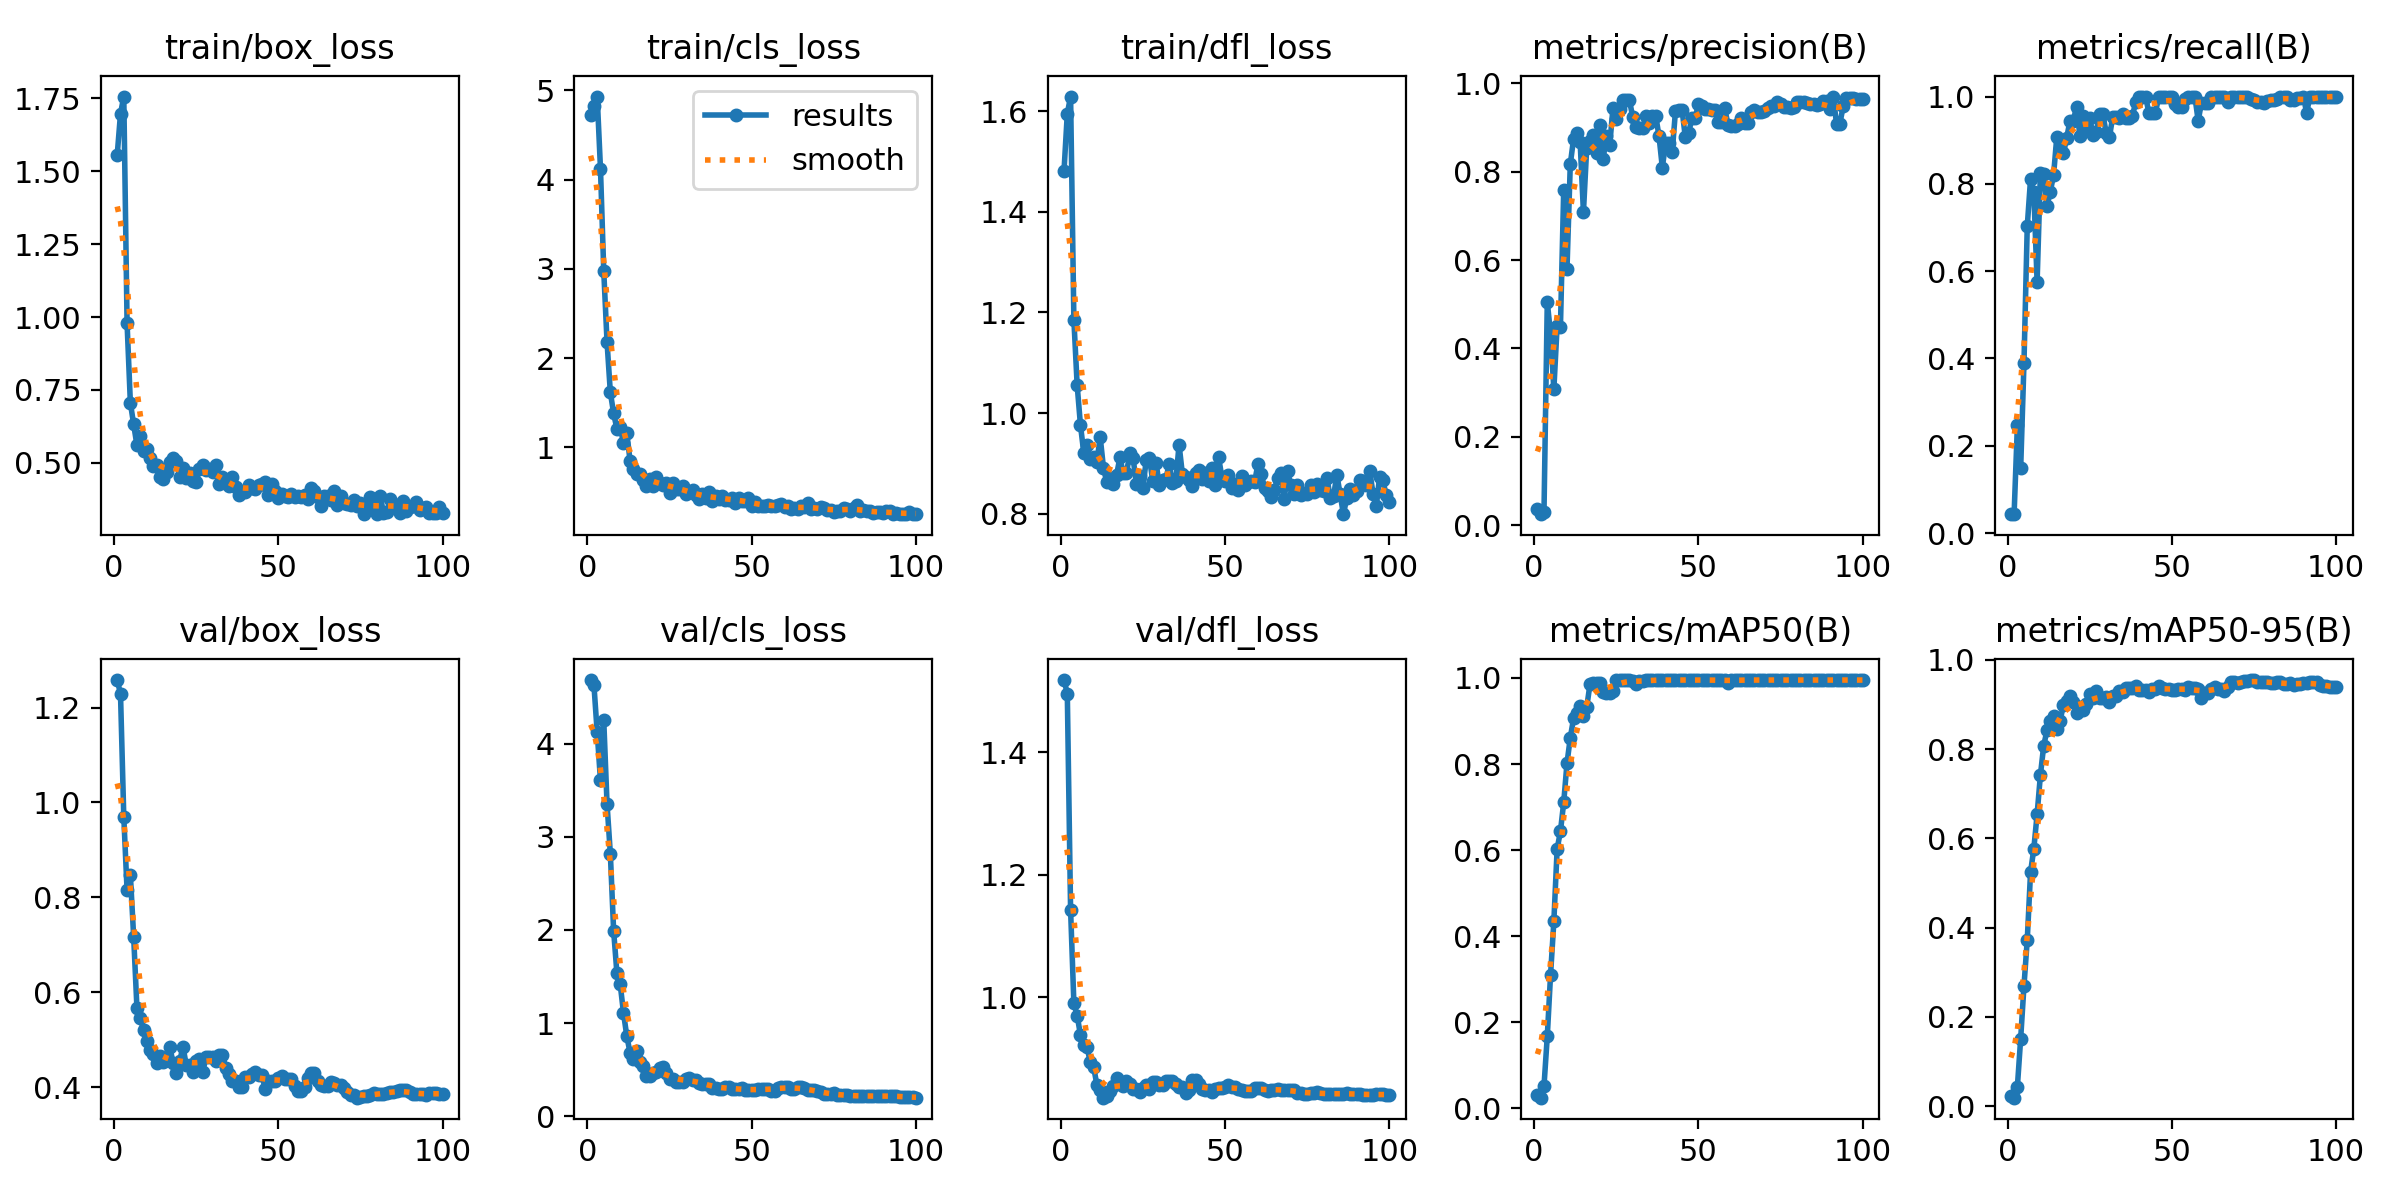
\includegraphics[width=0.80\textwidth]{imagens/results_ultimo_modelo.png}
    \caption{Gráficos de desempenho do segundo (e último) modelo criado para o Pokémon HeartGold.}
    \label{fig:results_ultimo_modelo}
\end{figure}

A partir das figuras \ref{fig:results_primeiro_modelo} e \ref{fig:results_ultimo_modelo} observa-se que:

\begin{itemize}
    \item As métricas de \textbf{precision} e \textbf{recall} estabilizaram-se mais rapidamente no último modelo, com valores superiores a 95\%, enquanto que no primeiro modelo estes valores oscilaram mais nas primeiras épocas.
    
    \item O \textbf{mAP@50} aproxima-se de 1.0 em ambos os modelos, no entanto, a convergência para esse valor é visivelmente mais rápida e estável no segundo modelo.
    
    \item O \textbf{mAP@50-95} é significativamente superior no segundo modelo, aproximando-se de 0.95, o que indica uma generalização muito mais eficaz, mesmo com critérios mais exigentes.
    
    \item As \textbf{perdas de treino e validação} diminuíram de forma mais acentuada no segundo modelo, mantendo-se baixas e estáveis ao longo do treino, sugerindo uma boa adaptação sem sinais de \textit{overfitting}.
\end{itemize}

% Matriz de confusão

Ao analisar as matrizes de confusão normalizadas das Figuras \ref{fig:confusion_matrix_primeiro_modelo} e \ref{fig:confusion_matrix_ultimmo_modelo}, observa-se um comportamento inesperado no segundo modelo (modelo final). Este apresenta uma matriz de confusão praticamente perfeita, sem registo de erros de classificação, o que, teoricamente, indicaria uma taxa de acerto de 100\% em todas as classes.

No entanto, na prática, durante os testes com o modelo em produção, foi possível verificar que este ainda comete alguns erros ocasionais, embora em pequena quantidade. Essa discrepância entre o desempenho observado na validação e o comportamento real pode estar relacionada com vários fatores, sendo os mais prováveis:

\begin{itemize}
    \item \textbf{Pouca diversidade no  conjunto de validação}: O conjunto de validação utilizado pode não representar de forma completa a variedade de situações e imagens reais enfrentadas pelo modelo em produção. Isso pode levar a uma avaliação artificialmente otimista.
    
    \item \textbf{Overfitting parcial ao conjunto de validação}: Mesmo que o modelo não mostre sinais evidentes de \textit{overfitting} nas métricas gerais, pode ter aprendido padrões muito específicos ao conjunto de validação, o que explicaria a performance quase perfeita nas métricas internas, mas um desempenho inferior em imagens não vistas anteriormente.
    
    \item \textbf{Imprecisão na anotação dos dados de produção}: As falhas observadas podem também estar relacionadas com diferenças nas condições visuais das imagens reais (luminosidade, resolução, sobreposição de elementos), que não estão refletidas nos dados de treino ou validação.
\end{itemize}

\begin{figure}[!h]
    \centering
    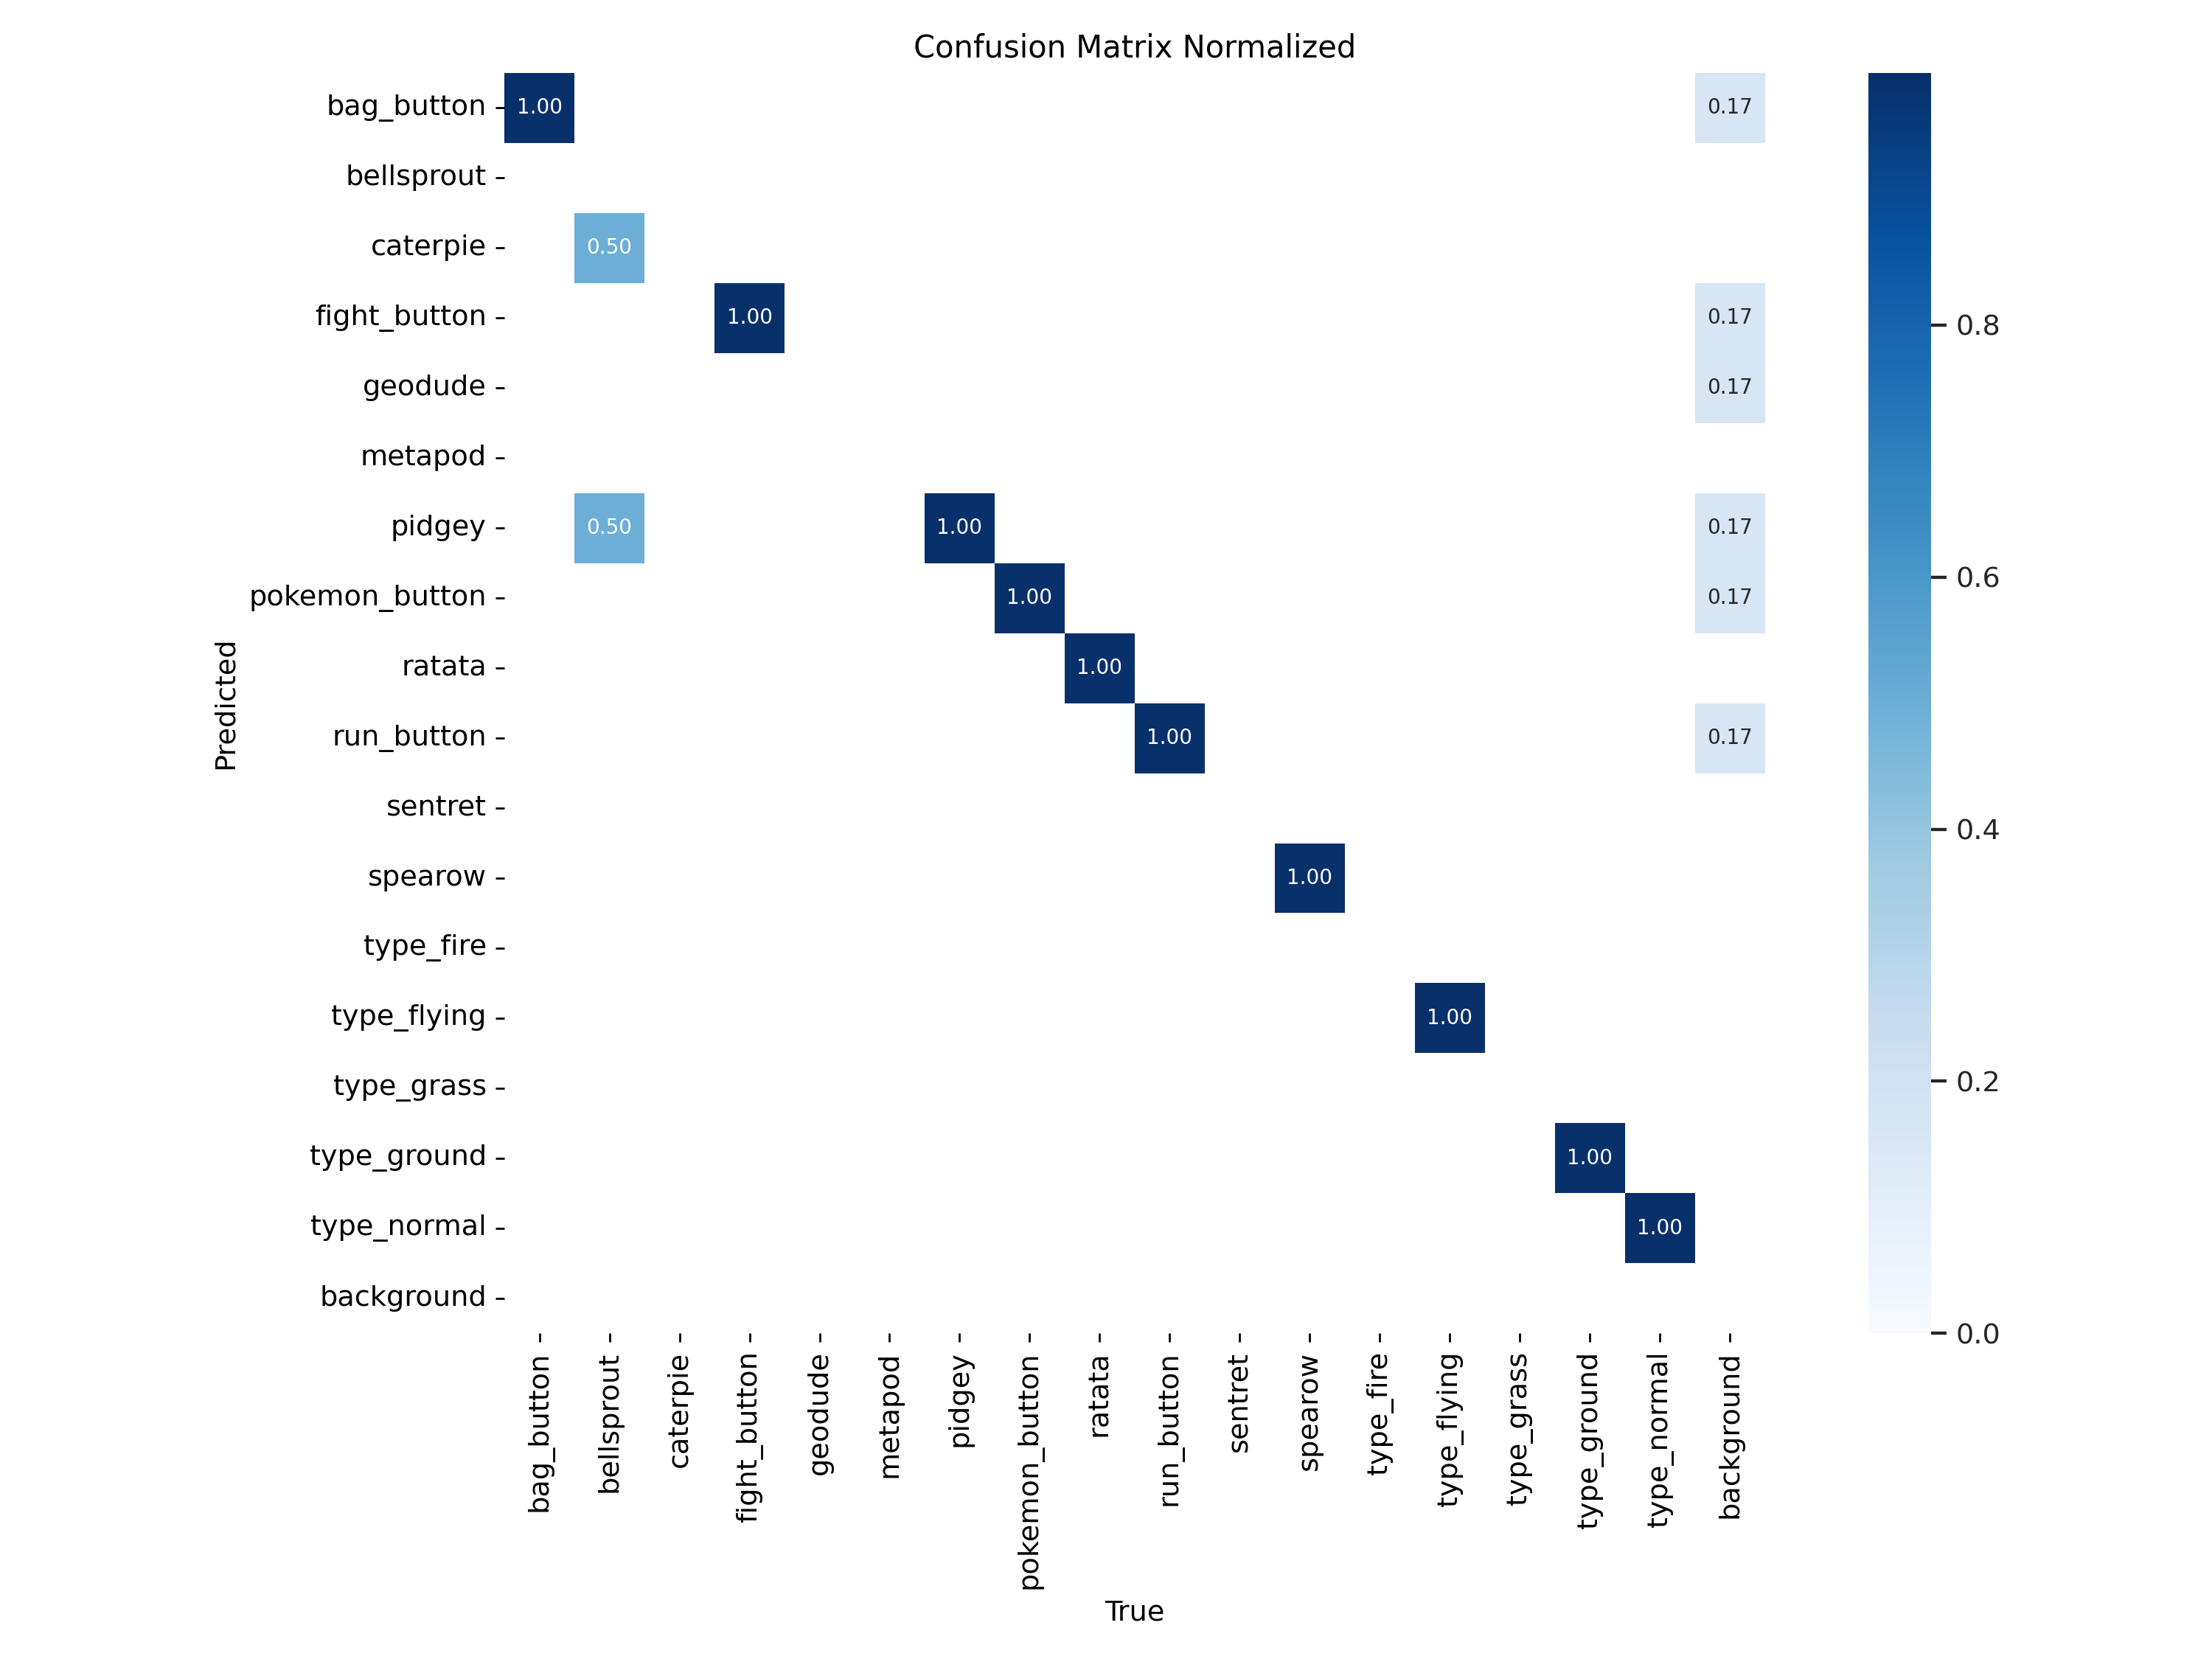
\includegraphics[width=0.65\textwidth]{imagens/confusion_matrix_normalized_primeiro_modelo.png}
    \caption{Matriz de confusão normalizada para o primeiro modelo criado para o Pokémon HeartGold.}
    \label{fig:confusion_matrix_primeiro_modelo}
\end{figure}

\begin{figure}[!h]
    \centering
    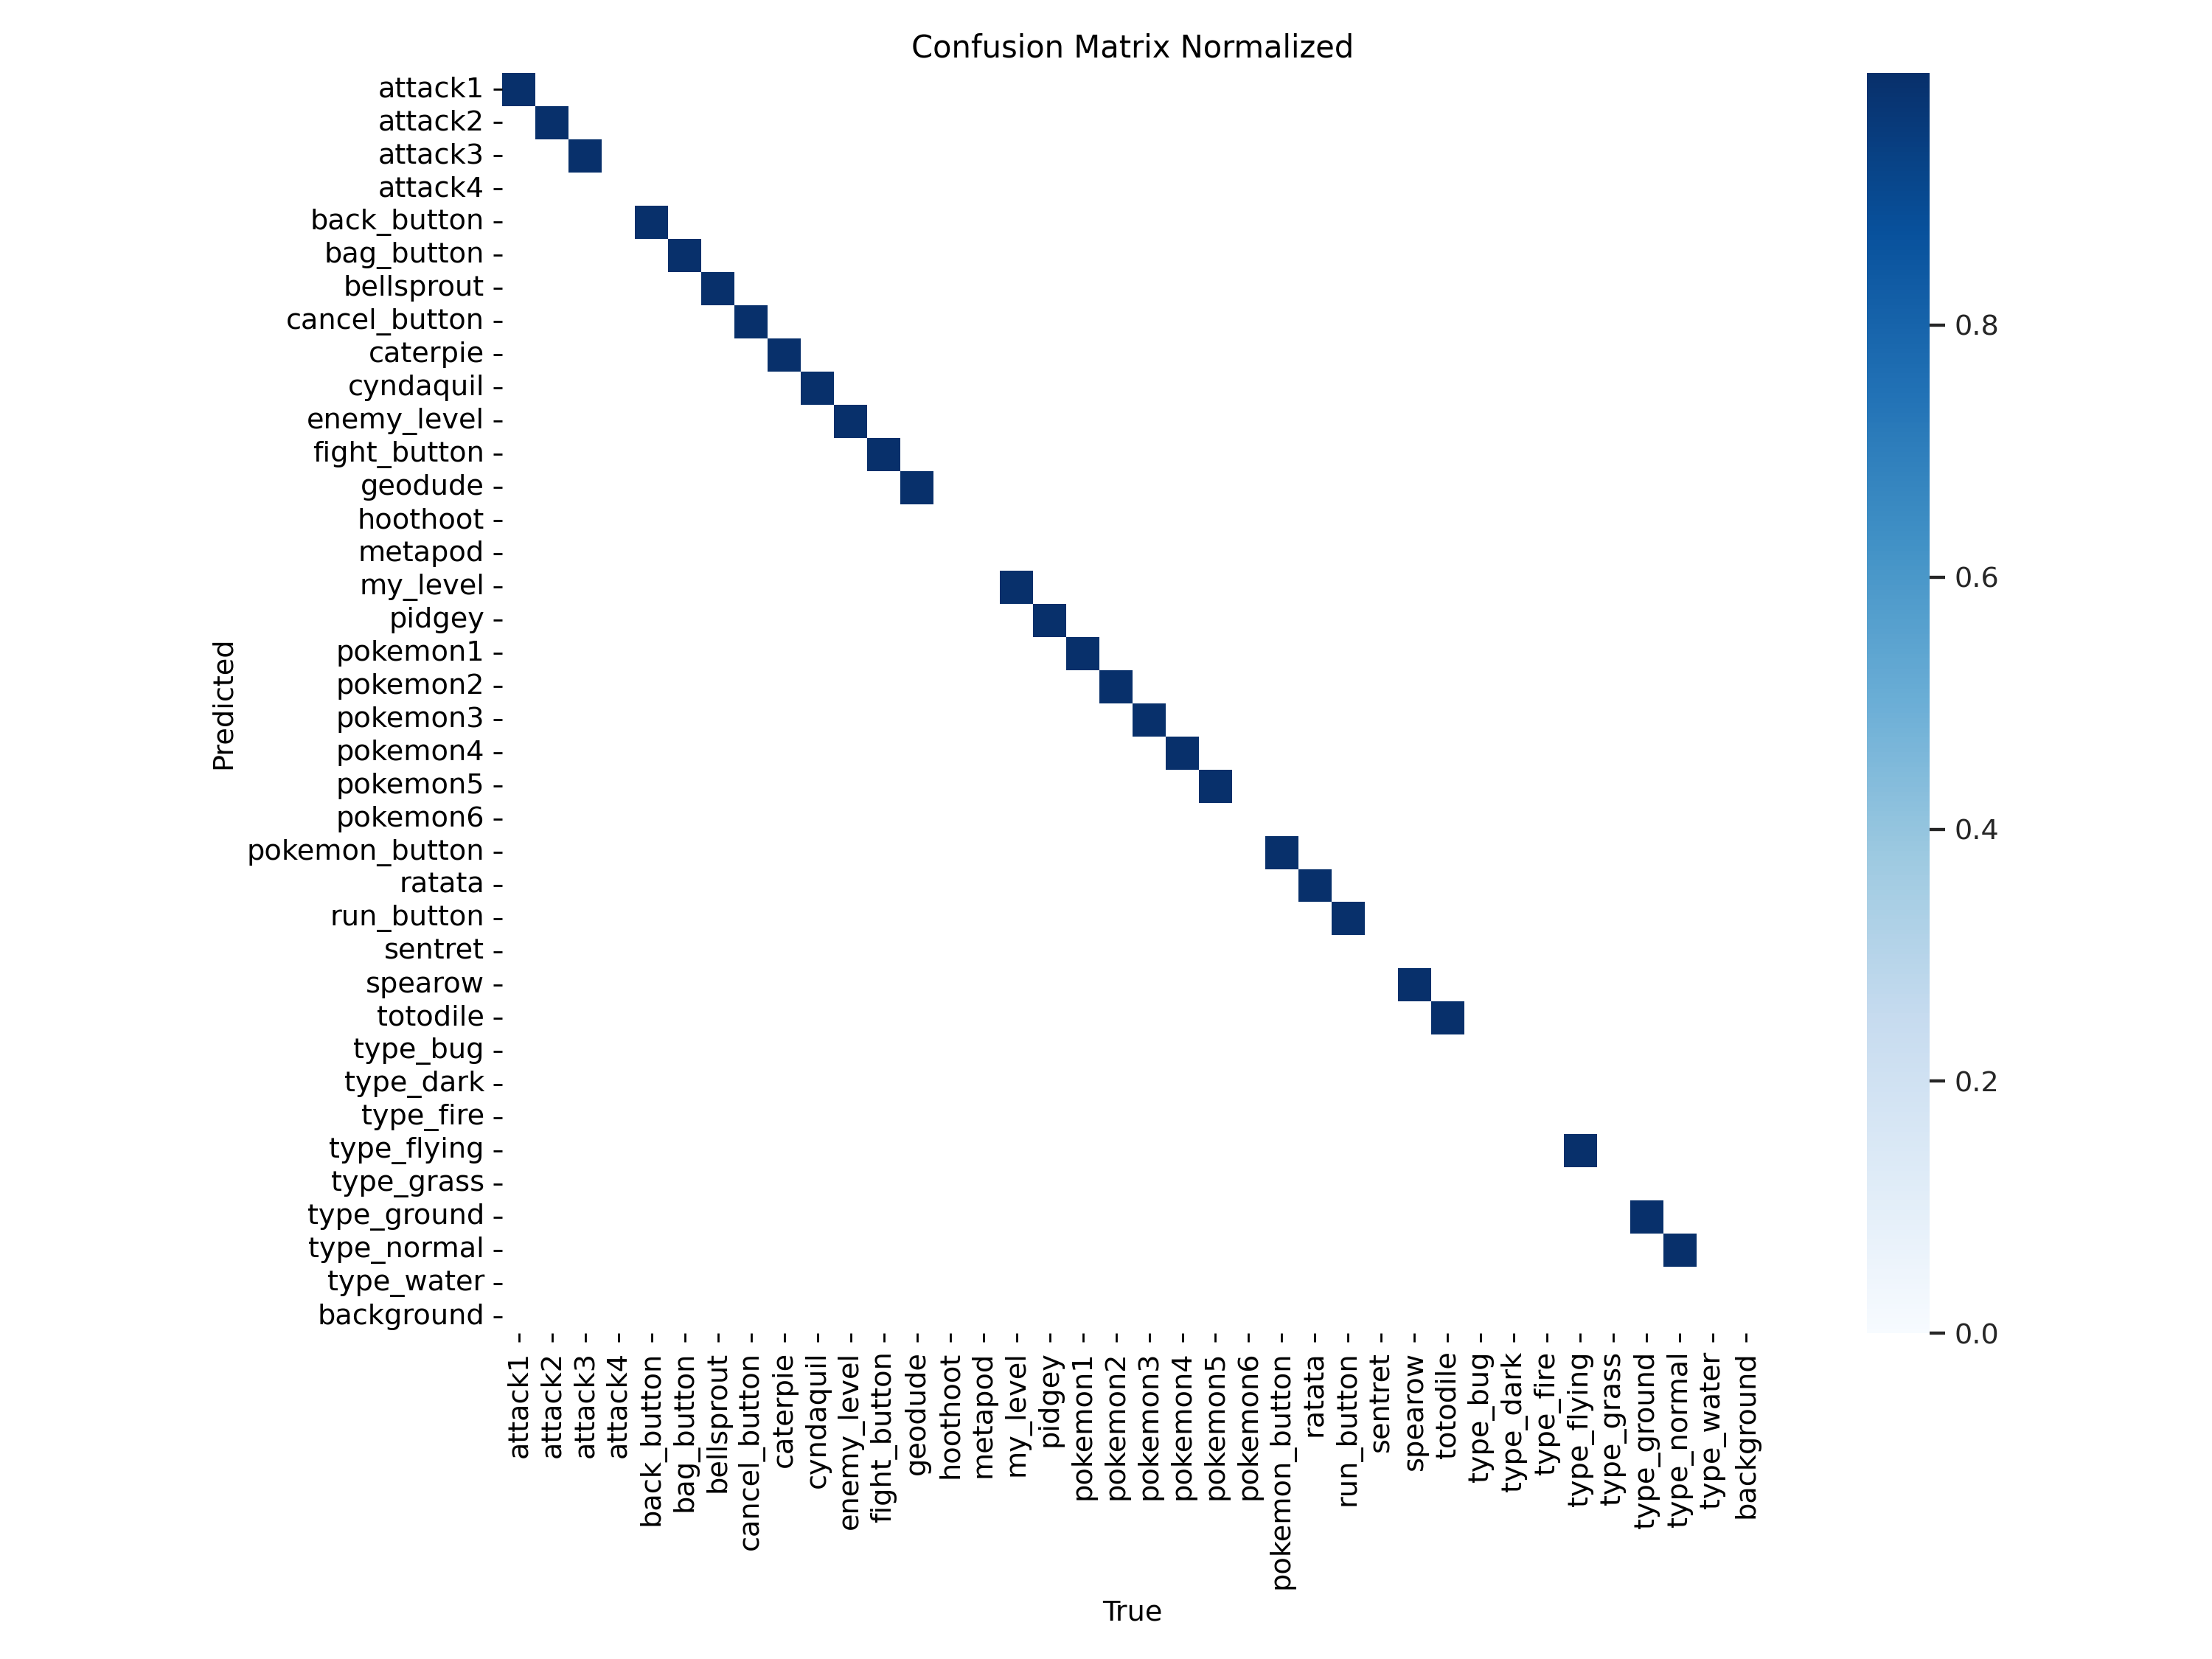
\includegraphics[width=0.80\textwidth]{imagens/confusion_matrix_normalized_segundo_modelo.png}
    \caption{Matriz de confusão normalizada para o último modelo criado para o Pokémon HeartGold.}
    \label{fig:confusion_matrix_ultimmo_modelo}
\end{figure}

Com base na análise das métricas obtidas, observa-se que o segundo modelo apresentou um desempenho significativamente superior, mesmo com um número maior de classes. No entanto, apesar dos resultados quase perfeitos apresentados nas matrizes de confusão normalizadas, é importante interpreta-las com cuidado, pois o facto destas indicarem uma taxa de acerto de 100\% pode não refletir com precisão o desempenho real do modelo em produção. Essa diferença pode estar relacionada com a limitada diversidade do conjunto de validação, possíveis padrões aprendidos especificamente para esse conjunto, ou diferenças nas condições reais de utilização.

Ainda assim, a evolução registada no último modelo em comparação ao primeiro é notável, provavelmente em grande parte devido à aplicação de técnicas de \textit{data augmentation}, que aumentaram a robustez do modelo e a sua capacidade de generalização a novas situações. Assim, justifica-se a escolha deste modelo como versão final para produção.

% Implementação em Produção
\section{Implementação em Produção} \label{implementacao_producao}
\subsection{Aplicação Desenvolvida}

A aplicação desenvolvida para produção foi construída em \textit{Python}, com uma interface gráfica implementada através da biblioteca \textit{Tkinter}.

Com o intuito de facilitar o processo de desenvolvimento do modelo final, decidiu-se que a aplicação não incluiria um modelo previamente definido e carregado automaticamente. Assim, para que a aplicação funcione corretamente, o utilizador deve selecionar manualmente o modelo pretendido, através de um botão localizado na barra de ferramentas da interface.

\begin{figure}[ht]
    \centering
    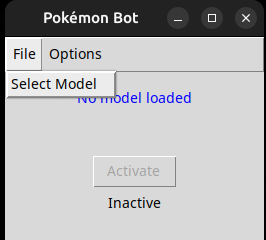
\includegraphics[width=0.3\linewidth]{imagens/carregamento_modelo.png}
    \caption{Interface principal da aplicação com o botão de carregamento do modelo}
    \label{fig:carregamento_modelo}
\end{figure}

De forma a tornar a aplicação mais flexível e reutilizável em outros contextos, foi ainda incluído um ecrã de configuração onde o utilizador pode personalizar algumas variáveis de funcionamento. As variáveis disponíveis para configuração são:

\begin{itemize}
    \item Intervalo de tempo entre capturas de ecrã (em milissegundos);
    \item Opção de guardar ou não as imagens capturadas;
    \item Opção de mostrar ou não na interface as imagens capturadas;
    \item Diretório onde as imagens capturadas serão armazenadas.
\end{itemize}

\begin{figure}[ht]
    \centering
    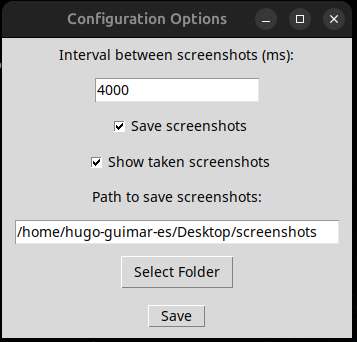
\includegraphics[width=0.4\linewidth]{imagens/configuracoes.png}
    \caption{Ecrã de configuração das variáveis da aplicação}
    \label{fig:configuracoes}
\end{figure}

Após o carregamento de um modelo, o botão de ativação da aplicação fica disponível. Quando ativada, a aplicação começa a capturar imagens do ecrã com a periodicidade definida, processa essas imagens através do modelo selecionado, e com base nos dados obtidos, move automaticamente o cursor do rato para interagir com a interface do jogo, selecionando as opções consideradas mais adequadas.

\begin{figure}[ht]
    \centering
    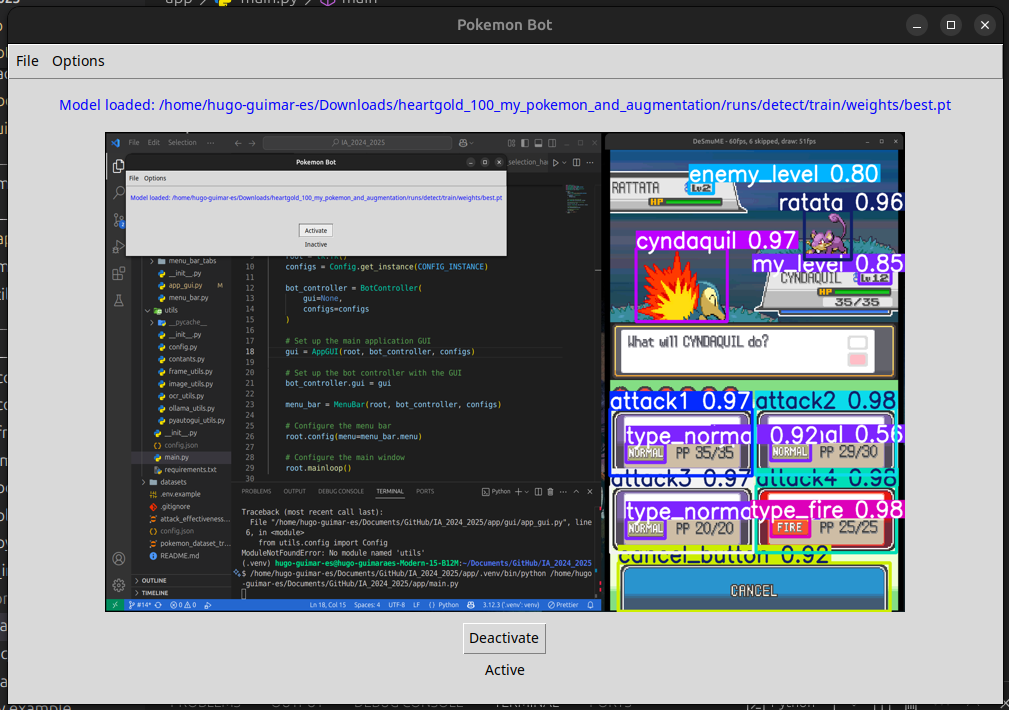
\includegraphics[width=1.0\linewidth]{imagens/aplicacao_em_execucao.png}
    \caption{Aplicação em execução após o carregamento do modelo}
    \label{fig:aplicacao_em_execucao}
\end{figure}

\subsection{Limitações da Aplicação}
Como foi utilizado um modelo de linguagem (LLM) e um reconhecimento ótico de caracteres (OCR) em produção, o bot acaba por demorar bastante tempo a executar as ações. Além disso, mesmo otimizando as instruções do modelo de linguagem, este continua a gerar respostas muito longas, o que, em alguns casos, obriga a executar o modelo novamente, uma vez que não foi possível interpretar a resposta anterior, atrasando ainda mais a tomada de decisão do bot.

Para realizar a movimentação automática do cursor, foi utilizada a biblioteca \textit{PyAutoGUI}. No entanto, esta funcionalidade pode apresentar limitações em determinados sistemas operativos.

No sistema operativo \textit{Windows}, poderá ser necessário executar o script com permissões de administrador, caso contrário, poderão ocorrer restrições na interação com o sistema.

Em sistemas \textit{Linux}, a aplicação poderá não funcionar corretamente se estiver a ser utilizado o servidor gráfico \textit{Wayland}, uma vez que este impõe fortes restrições quanto à interação entre aplicações. Para garantir o funcionamento da aplicação, recomenda-se a utilização do servidor gráfico \textit{Xorg} ou de uma outra alternativa que não seja tão restritiva.



% Conclusion
\section{Conclusão} \label{conclusao}
Olhando em retrospetiva, consideramos que o trabalho realizado foi bem concebido, tendo sido possível cumprir com os objetivos propostos, além de acrescentar funcionalidades que inicialmente não estavam previstas. Este projeto permitiu-nos aprofundar conhecimentos em áreas como visão computacional, integração de modelos de inteligência artificial e automação de tarefas baseadas em deteção e interpretação visual.


Mesmo com um trabalho bem concebido, temos a consciência que ainda poderia melhorar em diversos aspetos, como por exemplo: 

A leitura do ecrã a partir do \textit{easyOCR} para além de ser bastante lenta, atrasando as ações do bot, é bastante ineficiente, lendo as palavras com bastantes erros, e em alguns casos nem sequer as consegue ler. Futuramente poderia ser treinado um modelo exclusivamente para fazer leituras, onde o treino do mesmo seria realizado tendo como base textos com a fonte original do jogo, reduzindo a quantidade de erros, e muito provavelmente reduzindo o tempo de espera pela leitura.

A implementação do modelo de linguagem \textit{mistral} surgiu como alternativa para contornar a ineficiência do \textit{easyOCR} na leitura do ecrã. Embora o modelo consiga interpretar os resultados, mesmo com erros, e responder com alguma coerência, ele partilha das mesmas limitações de desempenho do \textit{easyOCR}. Além de ser bastante lento, muitas vezes não cumpre corretamente o prompt fornecido, gerando respostas excessivamente longas, o que atrasa o processo e exige múltiplas execuções devido à dificuldade em interpretar a resposta anterior. Para tentar reduzir o tempo das respostas foi implementada uma cache onde é guardado o promp respetivamente com a resposta dada pelo modelo, mas mesmo assim é preciso esperar no mínimo uma vez pela resposta do modelo. 

Como a versão do \textit{mistral} utilizada está otimizada para computadores mais limitados, a mesma apresenta várias lacunas no conhecimento, tomando muitas vezes decisões pouco coesas com o contexto da batalha.

Em suma, este projeto permitiu-nos consolidar conhecimentos teóricos e práticos, ao mesmo tempo que revelou oportunidades claras de melhoria, quer ao nível da performance técnica, quer na escolha das ferramentas utilizadas. Os próximos passos devem focar-se na melhoria da robustez e da adaptabilidade do sistema, de modo a alcançar um desempenho ainda mais fiável em cenários reais.


\end{document}
